\chapter{Cilvēku plūsmas analīze}
\section{Klasiskie mašīnmācīšanās algoritmi}
\paragraph{Lineārā regresija}
\hfill\par
Iespējams vienkāršākais un vislabāk aprakstītais statistikas un mašīnmācīšanās algoritms ir lineārā regresija. Lineārās regresijas reprezentācija ir vienādojums, kas apraksta līniju, kura vislabāk parāda attiecības starp ievades mainīgajiem \textit{x} un izvades mainīgajiem \textit{y}. Sakarību kas paskaidro \textit{x} un \textit{y} nosaka mainīgie, ko sauc par koeficientiem \textit{b} un tos izmanto kā svarus ievades datiem.

\begin{figure}[h]%
	\centering
	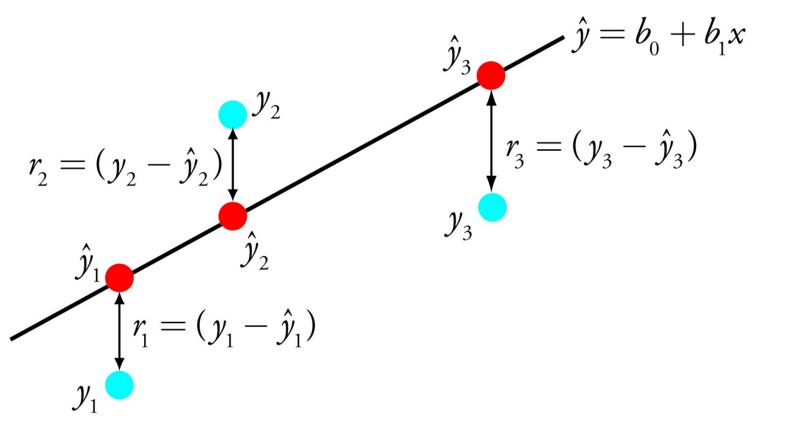
\includegraphics[height=4cm]{images/linreg.png} %
	\caption{Lineārās regresijas piemērs}%
	\label{fig:example}%
\end{figure} 

Par piemēru ņemot vienādojumu: $ y = b_0 + b_1 * x $ , tiek prognozētas \textit{y} vērtības, ņemot vērā \textit{x} vērtības un mērķis ir atrast koeficientus $b_0$ un $b_1$. Lai aprēķinātu lineārās regresijas modeli no šādiem datiem, gadiem ejot, ir parādījušās dažādas metodes, piemēram, lineārās algebras risinājumi vai gradienta nolaišanas optimizācija. Lineāro regresiju izmanto jau 200 gadu un ir tā ir bagātīgi pētīta. Šo tehniku var izmantot, lai, piemēram, atmestu datos esošus, līdzīgus mainīgos vai, lai noņemtu datiem troksni. 
\newpage
\paragraph{Atbalsta vektoru mašīnas}
\hfill\par
Atbalsta vektoru mašīnas (no angļu val. \textit{support vector machines}) (SVM) ir viens no vispopulārākajiem mašīnmācīšanās algoritmiem, klasifikācijas problēmu risināšanai. Svarīgs parametrs SVM ir hiperplakne (no angļu val. \textit{hyperplane}). Hiperplakne ir līnija, kas sadala ievades datus. To izvēlas tādu, lai tā vislabāk sadalītu ievades datus klasēs. Kā piemēru ņemot divdimensiju plakni, hiperplakni var vizualizēt kā līniju un perfektā gadījumā šī līnija pilnīgi atdalīs visus punktus pa klasēm. SVM algoritmi meklē koeficientus, kurus izvēloties hiperplakne vislabāk atdalīs klases. 
\begin{figure}[h]%
	\centering
	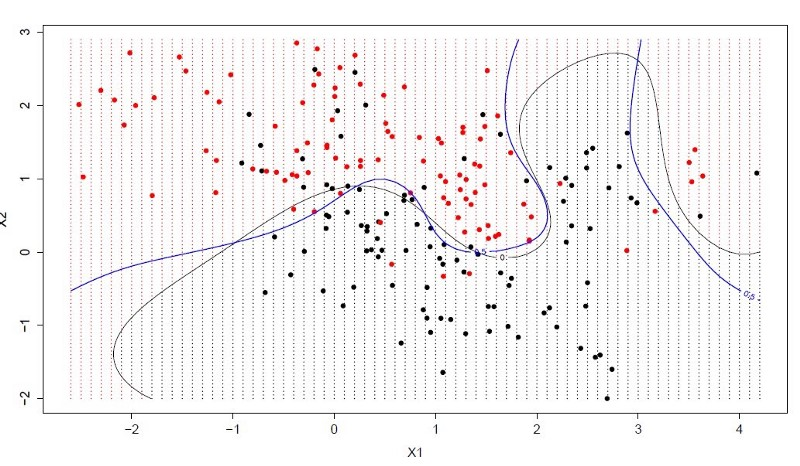
\includegraphics[height=5cm]{images/svm.png} %
	\caption{Atbalsta vektoru mašīnas piemērs}%
	\label{fig:example}%
\end{figure} 

Distance starp hiperplakni un tuvākajiem katras klases datu punktiem sauc par robežu (no angļu val. \textit{margin}). Hiperplakni uzskata par optimālu, kad izvēlētā līnija ir atdalījusi klasi un starp hiperplakni un datu punktiem ir vislielākā iespējamā robeža. Punkti, kas atrodas uz robežas veido atbalsta vektorus. Atbalsta vektori ir galvenā sastāvdaļa ko izmanto hiperplaknes definēšanai un klasifikatora izveidei.
\paragraph{Lēmumu koki}
\hfill\par
Lēmumu koki atspoguļo reālās dzīves koka struktūru un tos izmanto gan klasifikācijas, gan regresijas problēmu risināšanā. Analizējot datus, lēmumu kokus var izmantot, lai vizuāli aprakstītu lēmumus un lēmumu pieņemšanu. Mašīnmācīšanās gadījumā, lēmumu kokus apraksta kā klasifikācijas kokus vai regresijas kokus (\textit{CART - Classification and Regression Trees}), atkarībā no veicamā uzdevuma.  Galvenā šo koku doma ir audzēt zarus, pieņemot lēmumus, kuras koka īpašības izvēlēties, zinot apstāšanās nosacījumu \cite{dectree}. Lai gan lēmumu koki nav vispopulārākais mašīnmācīšanās veids, tas tiek pielietots klasifikācijas problēmu risināšanai dotajos pētījumos \cite{dectreepaper,pal2003assessment}.

\paragraph{Ģenētiskie algoritmi}
\hfill\par
Ģenētiskie algoritmi ir vēl viens algoritmu veids, kuru ir vērts izcelt. Tie ir algoritmi, kuri tiek izveidoti, balstoties uz notikumiem, kurus novēro dabīgajos evolūcijas procesos. Datorzinātnē ģenētiskie algoritmi ir optimizācijas algoritmi, kuri prot patstāvīgi apgūt jaunu informāciju, balstoties uz evolūcijas jēdzieniem kā dabīgā atlase un ģenētika. Ģenētisko algoritmu pamatideja ir simulēt Čārlza Dārvina piedāvāto teorēmu "izdzīvo stiprākais". Risinot problēmu, ģenētiskais algoritms saglabā tikai spēcīgākos indivīdus katrā paaudzē. Šie indivīdi sacenšas par resursiem un iespēju veidot nākamo paaudzi. Jaunās paaudzes tiek veidotas izvēloties vecākus no iepriekšējās paaudzes, veicot \textit{crossover} operāciju un mutāciju. Spēcīgākie indivīdi katrā paaudzē izveidos vairāk pēcnācēju nekā vājie indivīdi, tādējādi katra nākamā indivīdu paaudze kļūs labāka, galu galā iegūstot labāko rezultātu problēmas risināšanai. Beigu nosacījumu nosaka pirms algoritma izpildes, parasti, tiek noteikts paaudžu skaits vai kāds labāko indivīdu rezultātu slieksnis, kuru pēcnācēju paaudze pārsniedz. Ģenētiskie algoritmi gan nespēj risināt klasifikācijas problēmas, bet tos var lietot kā optimizācijas funkciju \cite{genopti} vai kā kārtošanas algoritmu \cite{deb2000fast}. Ģenētiskos algoritmus var izmantot lai aprēķinātu neironu tīklu svarus \cite{genalg}.
\begin{figure}[h]%
	\centering
	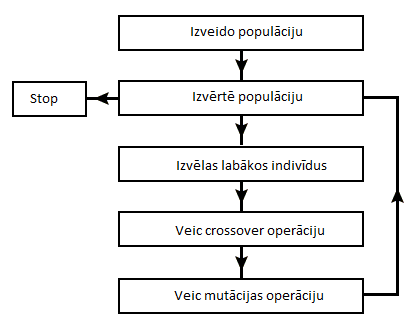
\includegraphics[height=6cm]{images/gen-algo-bilde.png} %
	\caption{Ģenētisko algoritmu modelis}%
	\label{fig:example}%
\end{figure}
\paragraph{Mākslīgie neironu tīkli}
\hfill\par
Mākslīgie neironu tīkli ir viena no populārākajām mašīnmācīšanās izmantotajām metodēm. Tas ir neapstrādāts elektronisks modelis, kas balstīts uz smadzeņu bioloģisko neironu tīklu. Var teikt, ka šāda neironu tīkla modelis, līdzīgi kā smadzenes, mācās no pieredzes. Teorētiski, šādu smadzeņu modelēšana, paredz, ka šāds mašīnmācīšanās risinājums, neprasa dziļas tehniskas zināšanas bioloģijā vai datorzinātnē, bet ir jāspēj tīklu izveidot pareizi kopā saliekot vairākas slāņu kārtas. Šādas, bioloģijas iedvesmotas metodes uzskata par nākamo lielo soli datorzinātnes industrijā \cite{staff}. \par
Iedziļinoties mākslīgo neironu tīklu uzbūvē, neironu tīkls sastāv no daudz, savstarpēji savienotiem mezgliem, kur katrs no mezgliem veic kādu matemātisku operāciju. To, ko atgriež katrs mezgls, nosaka matemātiskā operācija, ko šis mezgls veic kā arī citi parametri, kas specifiski šim mezglam. Šie mezgli galu galā tiek grupēti un šos mezglu grupējumus sauc par slāņiem (no ang. val. - \textit{layer}). \par
Mākslīgie neironu tīkli satur sava veida "mācīšanās likumus", kas ir process, kad tiek mainīti mezglu savienojumu svari atkarībā no informācijas ievadē. 
Kad neironu tīkls ir apmācīts tik tālu, ka lietotājs ir apmierināts, tad tīklam var sākt piedāvāt datus, kuri tad iziet cauri visiem slāņiem, tādā veidā turpinot mācības uz sākumā izveidotā modeļa bāzes. Neironu tīklus ir arī iespējams pārtrenēt, kas nozīmē, ka tīkls atpazīst tikai vienu ienākošo datu tipu. Ja tā notiek, tad mācīšanās vairs nav iespējama. Mākslīgos neironu tīklus izmanto dažādu problēmu risināšanai, piemēram, rakstu zīmju atpazīšanai \cite{nnchars}, attēlu kompresēšanai \cite{dony1995neural} vai pat akciju tirgus analizēšanai \cite{kimoto1990stock}. Šī darba nolūkos autors neironu tīklus izmantos dziļajai apmācībai.

\begin{figure}[h]%
	\centering
	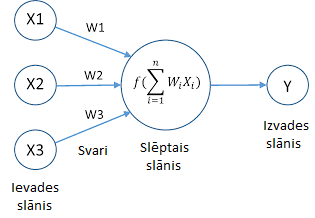
\includegraphics[height=4cm]{images/neironutikls.png} %
	\caption{Vienkāršs neironu tīkla modelis}%
	\label{fig:example}%
\end{figure}
\section{Dziļā mašīnmācīšanās, izmantojot konvolūcijas neironu tīklus}
Mašīnmācīšanās no dziļās mašīnmācīšanās atšķiras ar to, ka mašīnmācīšanās ir sarežģīti izmantot ļoti lielas datu kopas, taču ar dziļās apmācības metodēm tas ir iespējams. Dziļās mašīnmācīšanās metodes atgriež jebkādas vērtības sākot ar skaitliskām vērtībām, beidzot ar elementiem kā attēli, teksts vai skaņa, taču parastās mašīnmācīšanās metodes spēj atgriezt tikai skaitliskas vērtības kā, piemēram, klasifikācijas indeksu vai kādas funkcijas rezultātu. Mašīnmācīšanās izmanto dažādus automatizētus algoritmus, kas iemācās modeļa funkcijas un paredz nākotnes darbības no padotajiem datiem, kamēr dziļā apmācībā izmanto neironu tīklus, kas laiž datus caur daudz apstrādes slāņiem, lai izšķirtu datu īpašības. Lielākā atšķirība, pēc autora domām, starp mašīnmācīšanos un dziļo mašīnmācīšanos ir tajā, ka dziļās mašīnmācīšanās metodes automātiski datos atrod svarīgās īpašības, kamēr mašīnmācīšanās algoritmos šīs īpašības ir manuāli jānorāda. 
\begin{figure}[h]%
	\centering
	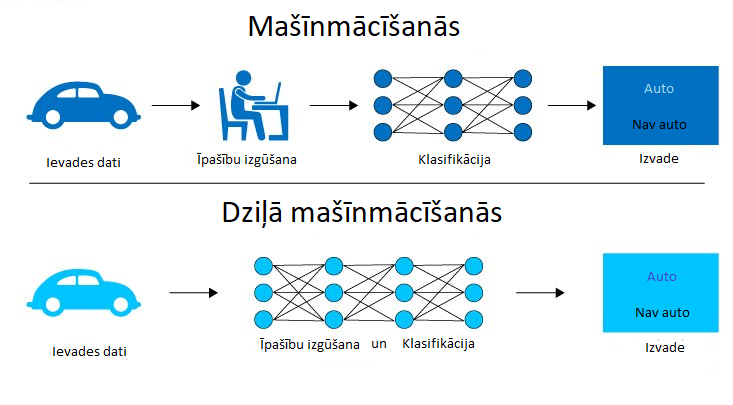
\includegraphics[height=7cm]{images/deeplearning.png} %
	\caption{Mašīnmācīšanās un dziļās mašīnmācīšanās salīdzinājums}%
	\label{fig:example}%
\end{figure}
Dziļā mašīnmācīšanās ļauj apmācīt matemātiskus modeļus, kas izveidoti no vairākiem datu apstrādes slāņiem, ar datiem, kas attēloti kā vairāku līmeņu abstrakcija (pētamā objekta galveno īpašību izdalīšana un mazsvarīgu aspektu ignorēšana). Šīs metodes ir uzlabojušas jaunākās tehnoloģijas balss atpazīšanā, objektu atpazīšanā attēlos, objektu detektēšanā. Dziļā mašīnmācīšanās, izmantojot atpakaļdatošanas algoritmus, sarežģītās datu kopu struktūrās meklē kā datoram vai jebkurai citai ierīcei būtu jāmaina iekšējie parametri starp tīklu slāņiem.

Īpašību apmācība ir metožu kopums, kas atļauj ierīcei padot neapstrādātus datus un automātiski iegūt īpašības, kas nepieciešamas, lai veiktu detektēšanu vai klasifikāciju. Dziļās mašīnmācīšanās metodes ir īpašību apmācības metodes ar vairākiem īpašību slāņiem, kurus iegūst apvienojot vienkāršus, taču nelineārus modeļus, kur katrs modelis pārveido īpašību no viena līmeņa uz augstāku, abstraktāku līmeni. Veicot pietiekami daudz šādus pārveidojumus, algoritmiem ir iespējams iemācīties ļoti sarežģītas darbības.\cite{deepnet} Darba ietvaros, datu klasifikācijai tiks izmantots konvolūciju neironu tīkls (\textit{CNN}), kas ir dziļās mašīnmācīšanās tips.

Konvolūcijas neironu tīkli (turpmāk \textit{CNN}) ir izveidoti, lai apstrādātu datus, kas ievadei padoti kā vairāki masīvi, piemēram, divdimensiju masīvi, kas satur pikseļu intensitātes vairākos krāsu kanālos (attēls). Vairākus datu veidus vienkāršojot, tos var izteikt kā masīvus: viendimensijas masīvs priekš signāliem vai skaitļu rindām, divdimensiju masīvi attēliem vai audio spektogrammām un trīsdimensiju masīvs video. Vislabāko rezultātu CNN tīklu veidi sasniedz risinot objektu detektēšanas \cite{li2015convolutional}\cite{matsugu2003subject}, segmentācijas \cite{long2015fully} vai klasifikācijas problēmas \cite{classif}\cite{krizhevsky2012imagenet}\cite{jia2014caffe}. Šī darba ietvaros CNN tiks izmantots objektu klasifikācijai.

\subsection{Tīklu slāņi}
Līdzīgi parastajiem neironu tīkliem arī konvolūciju neironu tīkli ir izveidoti no vairākiem slāņiem. CNN ir sarežģītāka struktūra kā parastam neironu tīklam. Vienkārša konvolūciju neironu tīkla arhitektūra sastāv no vairākiem, secīgi novietotiem slāņiem, kurus var izdalīt pa tipiem: konvolūcijas slānis (no kurienes arī rodas tīkla nosaukums), nelinearitātes slānis jeb aktivizācijas slānis, apvienošanas slānis un pilnīgi savienotais slānis (līdzīgi kāds tiek izmantots parastajos neironu tīklos). 
\subsubsection{Konvolūcijas slānis}
Konvolūcijas slānis ir CNN galvenā sastāvdaļa. Kā jau no nosaukuma var noprast, konvolūcijas slānī tiek veikta konvolūcijas operācija. Tiek izvēlēts filtrs (kernelis), un šis filtrs tiek pārvietots pāri masīvam (kas var būt gan attēls, gan audio, gan video) un katrā pozīcijā veic konvolūcijas operāciju. No konvolūcijas operācijas iegūtās vērtības tiek saskaitītas un rezultātā iegūts viens skaitlis. Kad konvolūcijas operācija tiek veikta visam masīvam, tiek iegūts masīvs, ko sauc par īpašību karti (no angļu val. \textit{feature map}) un jo vairāk filtrus izmanto, jo dziļāks kļūst attēls. Izmantojot 32x32x3 ievades masīvu un 5x5x3 filtru (filtram jābūt tikpat dziļam, cik dziļš ir ievades masīvs, lai būtu iespējams veikt matricu reizinājumu) tiks iegūta 28x28x1 īpašību karte un jo vairāk filtri tiks pielietoti, jo dziļāka būs šī īpašību karte un vairāk īpašības būs iespējams atrast masīvā. 
\begin{figure}[h]%
	\centering
	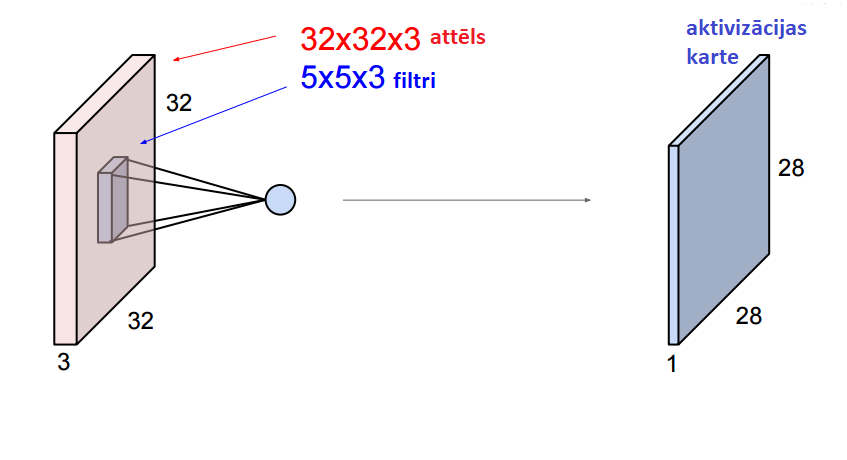
\includegraphics[height=4cm]{images/ActivationMap.png} %
	\caption{Konvolūcijas operācija pirmajā solī pielietojot 5x5 izmēra filtru}%
	\label{fig:example}%
\end{figure}

Šī īpašību karte satur informāciju par to kur atrodas minētās īpašības un cik labi šīs īpašības iedarbojas ar filtru, tādējādi norādot cik ļoti katrā masīva punktā atrodas ar filtru raksturotais elements. Pirms konvolūcijas operācijas veikšanas, ir nepieciešams izvēlēties trīs lielumus, kas ietekmēs īpašību karti:

\begin{itemize}
	\item \textbf{Dziļums} - atbilst filtru skaitam, kas izvēlēts konvolūcijas operācijas veikšanai. Ja ar masīvu tiks veikta konvolūcijas operācija ar trīs dažādiem filtriem, tad tiks atgrieztas trīs dažādas īpašību kartes, kuras būs apvienotas vienā trīs dimensiju masīvā ar dziļumu trīs.
	\item \textbf{Solis} - norāda par cik pikseļiem ievades masīvā pārvietosies filtra masīvs. Piemēram, ja konvolūcijas operāciju veic attēlam un solis ir divi, tad filtri neiet cauri katram pikselim, bet katram otrajam sākot no attēla augšējā kreisā stūra. Jo lielāks solis, jo mazākas būs īpašību kartes, kas ir noderīgi, ja tiek izmantoti lieli vai arī daudz filtru. Tādējādi, ir iespējams ietaupīt skaitļošanas resursus. 
	\item \textbf{Nulles-apdare} (no angļu val. \textit{zero-padding}) - tiek izmantota, ievades matricai pieliekot nulles vērtības ap robežām, lai šiem robežu elementiem būtu pilnībā iespējams pielietot filtrus. Nulles-apdares labās īpašības var izmantot arī lai mainītu īpašību kartes izmērus. Izmantojot nulles-apdari, šis process tiek dēvēts par plato konvolūciju (no angļu val. \textit{wide convolution}), bet nulles-apdares neizmantošanu sauc par šauro konvolūciju (no angļu val. \textit{narrow convolution}). 
	\begin{figure}[h]%
		\centering
		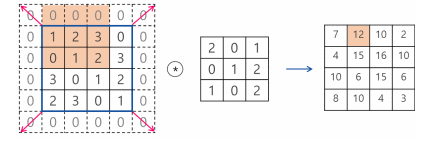
\includegraphics[height=2.5cm]{images/zero-padding.png} %
		\caption{Nulles-apdares piemērs \cite{zerpad}}%
		\label{fig:example}%
	\end{figure}
\end{itemize}
\subsubsection{Nelinearitātes slānis}
Nelinearitātes slānis konvolūciju neironu tīklos satur aktivizācijas funkciju, kas ņem no konvolūcijas operācijas atgriezto īpašību karti un izveido aktivizācijas karti. Aktivizācijas funkcija veic matricas elementu reizinājumu izmantojot saņemtos datus, kas nozīmē, ka tiek izvadīts tik pat liels masīvs, cik bija saņemts ievadē. Aktivizācijas funkciju tradicionāli implementē kā sigmoīdu vai hiperbolisku tangensa funkciju un tās galvenais mērķis ir novērst linearitāti. Nesenāki pētījumi gan norāda, ka konvolūcijas neironu tīklos rektificētas lineārās vienības (no angļu val. \textit{rectified linear units}) (ReLUs) strādā labāk kā tradicionālās aktivizācijas funkcijas \cite{nair2010rectified}. 
\begin{figure}[h]%
	\centering
	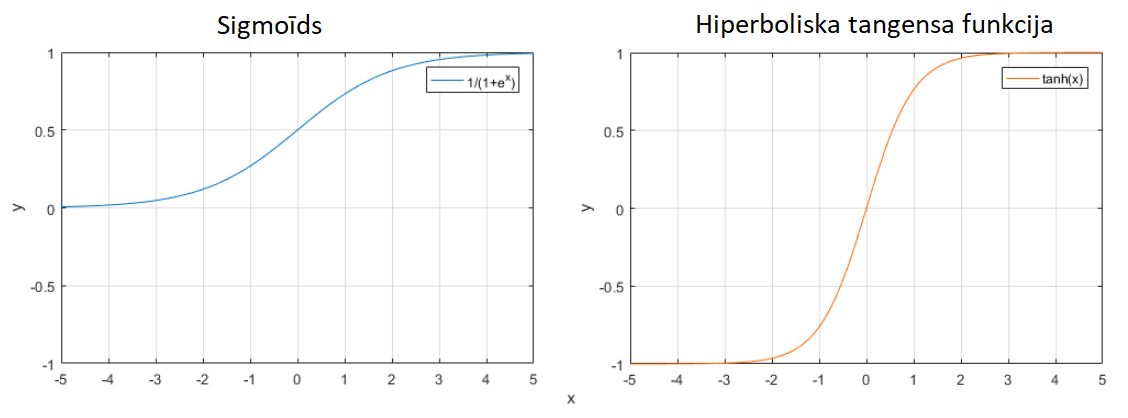
\includegraphics[height=4cm]{images/sigmoidhiperbol.png} %
	\caption{Sigmoīds un hiperboliskā tangensa funkcija ir populāri\\ izmantotas aktivizācijas funkcijas konvolūcijas neironu tīklos}%
	\label{fig:example}%
\end{figure}

Rektificētās lineārās vienības (ReLUs) ir speciāla implementācija, kas apvieno nelinearitātes un rektifikācijas slāņu (rektifikācijas slānis atgriež ievades datu elementu moduli) operācijas konvolūcijas neironu tīklos. Rektificēta lineāra vienība ir gabalveida (no angļu val. \textit{piecewise}) lineāra funkcija, kas definēta sekojoši:
\[ Y_i^{(l)} = max(0,Y_i^{(l-1)}) \]
\begin{figure}[h]%
	\centering
	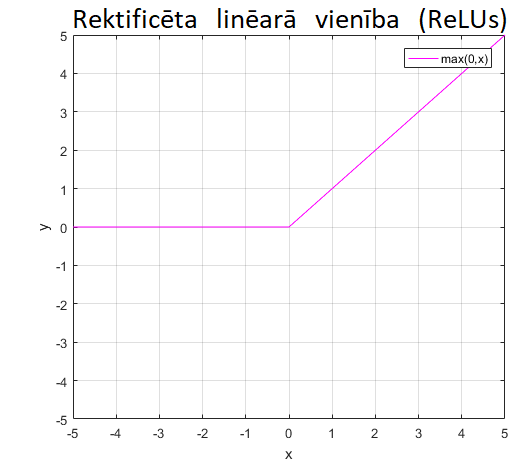
\includegraphics[height=4cm]{images/relu.png} %
	\caption{Rektificēta lineāra vienība}%
	\label{fig:example}%
\end{figure}

Konvolūcijas neironu tīklos, ReLUs ir trīs nozīmīgas priekšrocības pār tradicionālajām loģistikas funkcijām (sigmoīds) vai hiperboliskajām tangensa aktivizācijas funkcijām:
\begin{itemize}
	\item ReLUs efektīvi izplata gradientu, kas samazina iespēju saskarties ar gradienta izzušanas problēmu, kas ir parasta problēma dziļajās neironu tīklu arhitektūrās \cite{hochreiter1998vanishing}.
	\item Īpašības karšu negatīvās vērtības, rektifikācijas lineārā vienība pārveido par nullēm, tādējādi tiekot galā ar anulēšanas problēmu (no angļu val. \textit{cancellation problem}) kā arī izvadē iegūtā aktivizācijas karte saturēs daudz izsētāku vērtību apjomu. Šāds vērtību izkaisījums nodrošina stabilitāti gadījumā, ja ievadē notiek nelielas izmaiņas, piemēram, troksnis\cite{glorot2011deep}. 
	\item Ņemot vērā skaitļošanas sarežģītību, ReLUs sastāv no ļoti vienkāršām operācijām, kas nozīmē, ka šīs operācijas smagi neietekmē CNN veiktspēju, kas padara to implementēšanu konvolūcijas neironu tīklos ļoti efektīvu.
\end{itemize}
Šo priekšrocību dēļ, lielākā daļa jaunāko konvolūcijas neironu tīklu arhitektūru, piemēram, \cite{krizhevsky2012imagenet}\cite{DBLP:journals/corr/HeZR015}\cite{simonyan2014very}, izmanto tieši rektificētās lineārās vienības kā aktivizācijas funkciju nelinearitātes slānī.
\subsubsection{Apvienošanas slānis}
Apvienošanas slāņa (no angļu val. \textit{pooling layer}) galvenā funkcija ir samazināt aktivizāciju karšu dimensiju skaitu. Lai samazinātu iespēju pārlieku apmācīt tīklus (no angļu val. \textit{overfitting}) un samazinātu nepieciešamos skaitļošanas resursus, visbiežāk, šis slānis tiek pielietots pēc vairāk citu slāņu operāciju veikšanas (piemēram, pēc vairākiem konvolūcijas un aktivizācijas slāņiem). Apvienošanas operācijas mērķis ir saglabāt jau atrastās īpašības mazākā attēlojumā. Šis mērķis tiek sasniegts atmetot mazsvarīgos datus, lai iegūtu labāku telpisko izšķirtspēju. 

Apvienošanas slānī tiek definēts filtrs, kurš katrā operācijas solī tiks reducēts līdz vienai vērtībai. Līdzīgi kā konvolūcijas slānī, tiek izvēlēts solis pēc cik pozīcijām atkal tiks pielietots apvienošanas filtrs. Kad filtrs ir izmantots visām iespējamajām masīva pozīcijām, izvadē tiek iegūta telpiski samazināta aktivizācijas karte.

Visbiežāk izmantotās redukcijas metodes ir maksimumu apvienošana vai vidējās vērtības apvienošana. Maksimuma apvienošanas filtri meklē vislielāko vērtību filtra reģionā un atmet pārējās vērtības. Vidējās vērtības apvienošanas filtri saglabā filtr reģiona vidējo vērtību. Maksimuma apvienošana demonstrē spēju ātrāk konverģēt salīdzinājumā ar vidējās vērtības apvienošanu un citām metodēm, tāpēc to izmanto visbiežāk \cite{scherer2010evaluation}. 
\begin{figure}[h]%
	\centering
	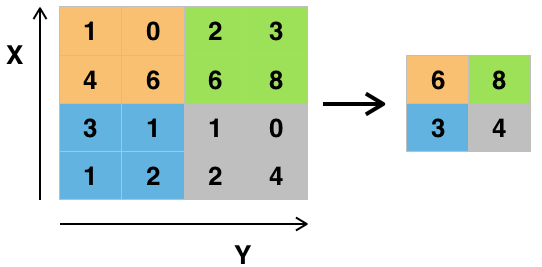
\includegraphics[height=3cm]{images/maxpool.png} %
	\caption{Vienkāršs maksimuma apvienošanas slāņa modelis \cite{maxpool}}%
	\label{fig:example}%
\end{figure}
\subsubsection{Pilnīgi savienotais slānis}
Pilnīgās savienošanas slāņa (no angļu val. \textit{fully connected layer}) galvenais uzdevums ir, izmantojot no iepriekšējiem slāņiem iegūto īpašību karti, sadalīt ievades datu masīvu pa klasēm, kas balstītas uz apmācībā izmantoto datu kopu. Papildu klasifikācijas funkcijai, pilnīgi savienotos slāņus ir vērts ievest tīklā, lai noskaidrotu īpašību karšu nelineārās kombinācijas. Šis slānis kā ievades datus saņem konvolūcijas, aktivizācijas vai apvienošanas slāņu izvadi un atgriež \textit{N} dimensiju vektoru, kur \textit{N} ir neironu tīklam piedāvāto klašu skaits. Šis klašu jeb atšķirīgu detektējamo objektu skaits ir jādefinē pirms tīkla apmācības. Iepriekš minētais vektors saturēs informāciju par to cik ļoti katrs aktivizācijas kartes elements korelē ar definētajām klasēm. Piemēram, ja tīklam ievadē ir padots attēls ar cilvēku, aktivizācijas kartē būs augstas vērtības īpašībām, kas raksturo, ka objektam ir divas rokas un divas kājas. Summējot no pilnīgi savienotā slāņa izvadē iegūtās varbūtības ir jāiegūst vērtība 1. To nodrošina \textit{Softmax} funkcija, ko izmanto kā aktivizācijas funkciju pilnīgi savienotajā slānī. \textit{Softmax} funkcijai kā ievades datus padod vektoru ar patvaļīgiem rezultātiem, kas iegūti pēc klasifikācijas un šī funkcija saspiež šīs vērtības vektorā, kur visas vērtības ir robežās no 0 līdz 1 un visa vektoru vērtību summa ir 1. \textit{Softmax} aktivizācijas funkcija ir definēta sekojoši:
\[f_j(z) = \frac{e^{z_j}}{\sum_k e^{z_k}} \]
Kur \textit{z} ir masīvs ar vērtībām, kas iegūtas pēc klasifikācijas.
\subsection{Tīklu arhitektūras}
Nav noteikts viens veids kādai ir jābūt pareizai konvolūcijas neironu tīkla struktūrai, taču ir pieņemts, ka konvolūcijas neironu tīkls vienmēr satur jau minētos tīkla slāņus. Mūsdienās, standarta CNN arhitektūru sāk aizvietot ar sarežģītākām tīklu arhitektūrām, kuras visbiežāk parastos četrus konvolūcijas neironu tīklu slāņus maina vietām un atkārto vairākas reizes. Izveidot pašam savu CNN struktūru nav sarežģīti, to pat var padarīt funkcionālu, taču, lai tas funkcionētu labāk kā jau esošās arhitektūras, ir nepieciešams ieguldīt daudz laika testēšanai un pētīšanai. Dotajā brīdī, ir pieejami tūkstošiem, un katru dienu parādās jaunas, konvolūcijas neironu tīklu arhitektūras, šī darba ietvaros ir vērts pieminēt dotās tīklu arhitektūras: \textit{AlexNet}, \textit{VGG Net}, \textit{GooGleNet} un \textit{ResNet}.

\subsubsection{AlexNet}

\textit{AlexNet} tīklu arhitektūru var uzskatīt par pirmo konvolūcijas neironu tīklu arhitektūru, kas uzrādija labus rezultātus, risinot objektu detektēšanas, klasifikācijas un lokalizācijas problēmas \cite{ILSVRC15}. Tā tika izveidota 2012. gadā un ir aprakstīta rakstā \textit{"ImageNet Classification with Deep Convolutional Networks"}\cite{krizhevsky2012imagenet}. 2012. gada ILSVRC (\textit{ImageNet Large-Scale Visual Recognition Challenge}) \textit{AlexNet} sacensībās uzrādīja tik labus rezultātus kā neviena CNN arhitektūra līdz šim \cite{ILSVRC15} un kopš šīm sacensībām CNN vispārīgi sāka gūt popularitāti objektu detektēšanā. 

Salīdzinājumā ar mūsdienu arhitektūrām, \textit{AlexNet} struktūra ir salīdzinoši vienkārša. Tīklā ir 5 konvolūcijas, apvienošanas slāņi un nelinearitātes slāņi un 3 pilnīgi savienotie slāņi. Nelinearitātes slānī tiek izmantota \textit{ReLU} aktivizācijas metode, jo testēšanas procesā, \textit{ReLU} apmācības laiki bija vairākas reizes mazāki, kā ierastajai hiperboliskajai tangensa aktivizācijas funkcijai. 
\begin{figure}[h]%
	\centering
	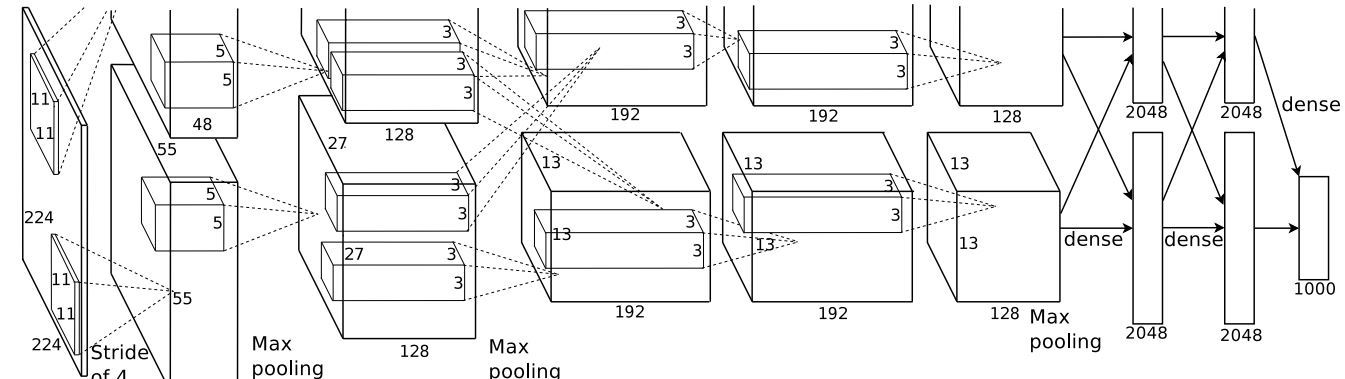
\includegraphics[height=4cm]{images/alexnet.jpg} %
	\caption{\textit{AlexNet} tīkla arhitektūra \cite{alexnetimage}}%
	\label{fig:example}%
\end{figure}
\subsubsection{VGG Net}
\textit{VGG Net} arhitektūra ir izveidota 2014. gadā un aprakstīta rakstā ar nosaukumu \textit{"Very deep convolutional networks for large-scale image recognition"}\cite{simonyan2014very}. Šīs arhitektūras galvenā īpašība ir vienkāršība un slāņu daudzums (no angļu val. \textit{depth}), saglabājot tīklu nesarežģītu. \textit{VGG Net} ir 19 slāņu konvolūcijas neironu tīkls, kas konvolūcijas slānī izmanto mazus, 3x3 izmēra filtrus ar soli 1 un 1 \textit{zero-padding} jeb nulles-apdares operāciju un apvienošanas slānī izmanto 2x2 filtrus ar soli 2.
Pēc tīkla arhitektūras autoru domām, lai gan 3x3 izmēru filtri ir mazi, divus filtrus ir iespējams apvienot (novietojot 2 konvolūcijas slāņus vienu pēc otra), simulējot 5x5 izmēra filtru un apvienojot 3 konvolūcijas filtrus tiks simulēts 7x7 filtrs. Vairāku filtru apvienošana dod iespēju iegūt lielāku filtra izmēru, saglabājot labās mazo filtru īpašības, piemēram, ar vairākiem konvolūcijas slāņiem, ir iespējams arī vairākas reizes pielietot \textit{ReLU} aktivizācijas funkciju. Izmantojot vairākus mazus filtrus, tīkls var iemācīties smalkākas, sarežģītākas īpašības būtiski neietekmējot skaitļošanas resursu izmantošanu.
\begin{figure}[h]%
	\centering
	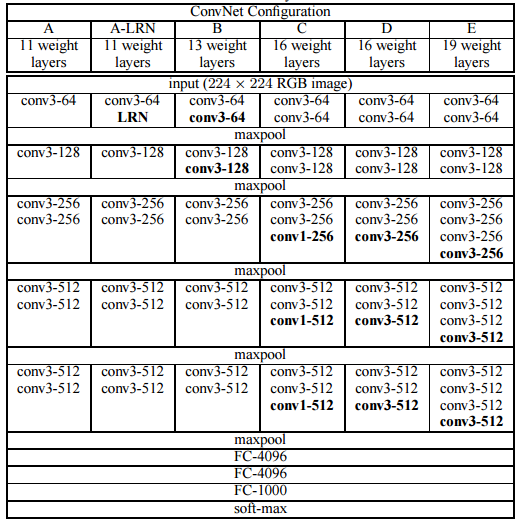
\includegraphics[height=7cm]{images/vggnet.png} %
	\caption{\textit{VGG Net} tīklu struktūras \cite{simonyan2014very}}%
	\label{fig:example}%
\end{figure}

\textit{VGG Net} arhitektūrā, pēc katra apvienošanas slāņa, konvolūcijas slāņos izmantotas filtru skaits dubultojas. Kā rezultātā datu telpiskais izmērs pēc konvolūcijas un apvienošanas slāņu operācijām samazinās, bet datu dziļums palielinās, kas ir rezultāts daudz filtru pielietošanai. Attēlā 1.10 ir parādīts, ka \textit{VGG Net} struktūra ir sadalīta blokos un katrā blokā konvolūcijas operācija, ar vienāda izmēra filtriem, tiek veikta vairākas reizes, lai iegūtu smalkākas īpašības.
\subsubsection{GoogLeNet}
Pretēji \textit{VGG Net} principam "vienkāršība un dziļums", \textit{GoogLeNet} arhitektūrai ir ļoti sarežģīta struktūra, kurā ir iebūvēti \textit{Inception} modeļi. \textit{GoogLeNet} 2015. gadā izveidoja kompānijas \textit{Google} pētnieki un aprakstīja tīkla arhitektūru rakstā "\textit{Going Deeper with Convolutions}" \cite{szegedy2015going}. \textit{GoogLeNet} arī uzvarēja 2014. gada ILSVRC sacensībās \cite{ILSVRC15}. Šī tīkla arhitektūra bija pirmā, kas novērsās no standarta metodēm: konvolūciju neironu tīklus kārtot slāņus secīgi, vienu pēc otra, piedāvājot slāņus kārtot paralēli.

\textit{GoogLeNet} arhitektūru sakārtojot secīgi, tā izmantotu milzīgus atmiņas apjomus un prasītu pamatīgus skaitļošanas resursus, taču, izmantojot \textit{Inception} modeļus, šo problēmu var samazināt.
\begin{figure}[h]%
	\centering
	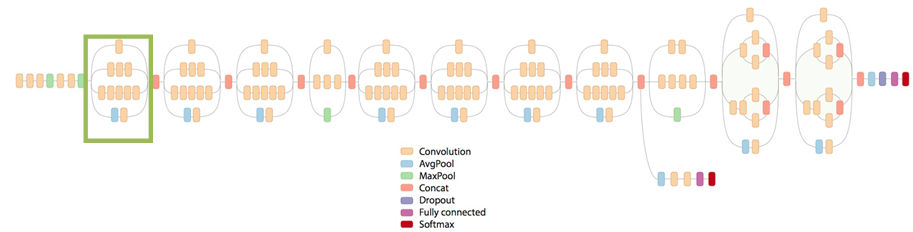
\includegraphics[height=4cm]{images/GoogLeNet2.png} %
	\caption{\textit{GoogLeNet} tīkla struktūra \cite{szegedy2015going}}%
	\label{fig:example}%
\end{figure}

Attēlā 1.11 var novērot, ka tīkla struktūra ir sadalīta moduļos (piemērs zaļā taisnstūrī) un šie moduļi satur blokus, kas ir novietoti paralēli viens otram. Katrs šis modelis ir \textit{Inception} modelis. Šis modulis ir kā vairāki konvolūcijas filtra ievades punkti, kurus apstrādā vienlaicīgi, paralēli, visus rezultātus pēc tam savieno, šādā veidā no katras ievades datu vienības tiek veikta vairāku līmeņu īpašību (\textit{feature}) izgūšana.

\begin{figure}[h]%
	\centering
	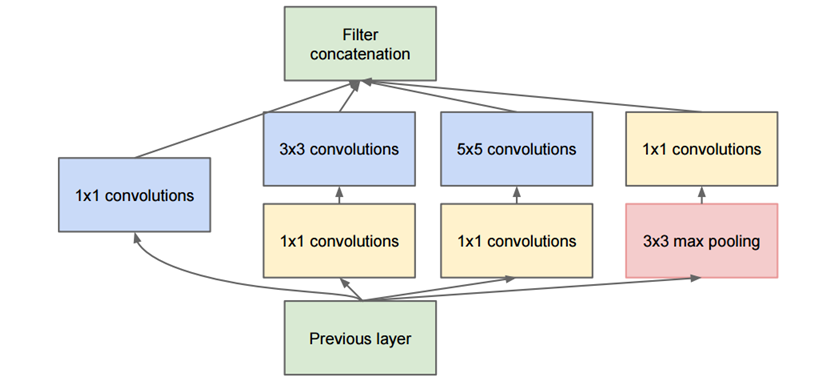
\includegraphics[height=4cm]{images/inception.png} %
	\caption{\textit{Inception} modelis \cite{szegedy2015going}}%
	\label{fig:example}%
\end{figure}

\subsubsection{ResNet}
No augstāk minēto arhitektūru aprakstiem, var izdarīt secinājumu, ka palielinot slāņu skaitu, palielināsies tīkla precizitāte (ja netiek pieļauta tīkla pār-apmācīšana (no angļu val. \textit{overfitting})). \textit{Microsoft} komandas, 2015. gadā izveidotā CNN arhitektūra ir 152 slāņu arhitektūra, kas uzstādīja jaunus rekordus klasifikācijā, detektēšanā un lokalizācijā, uzvarot 2015. gada ILSVRC sacensībās \cite{ILSVRC15}. 

Neskaitot lielo slāņu skaitu,    \textit{ResNet} tīklu struktūra no pārējām, jau minētajām, arhitektūrām atšķirt tas, ka \textit{ResNet} sastāv no "atlikumu blokiem" (no angļu val. \textit{residual blocks}). Šo bloku galvenā doma ir saglabāt tajā padoto informāciju un pievienot to izejošajai informācijai, nevis pilnībā aizmirst ievades datus kā tas notiek citās arhitektūrās \cite{he2016deep}. 

\begin{figure}[h]%
	\centering
	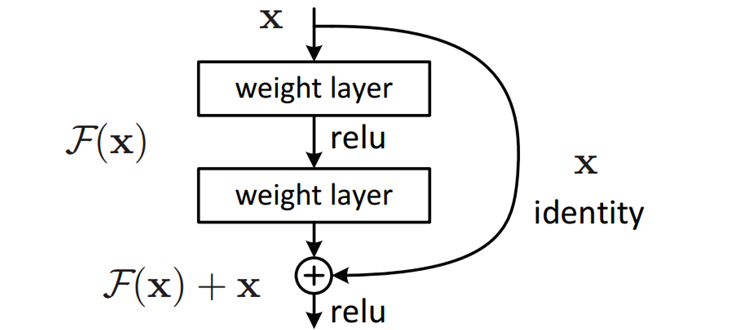
\includegraphics[height=4cm]{images/resnet.png} %
	\caption{\textit{ResNet} atlikumu bloks \cite{he2016deep}}%
	\label{fig:example}%
\end{figure}
\subsection{Ietvari un programmatūra}
Dziļās mašīnmācīšanās nozarē joprojām ir ļoti daudz ko pētīt un atklāt, kas nozīmē, ka lielākajām tehnoloģiju kompānijām kā \textit{Google}, \textit{Amazon}, \textit{Facebook} un \textit{Microsoft} ir vēlme būt labākajiem dziļās mašīnmācīšanās risinājumu izstrādātājiem. Visām minētajām kompānijām ir aktuāli izstrādāt viņu pašu dziļās mašīnmācīšanās ietvarus vai atbalstīt jau esošus risinājumus. Pieņemot, ka ir simtiem dziļās mašīnmācīšanās risinājumu, ir aktuāli apskatīt dažus no visbiežāk izmantotajiem ietvariem.

\subsubsection{\textit{TensorFlow}}

\textit{TensorFlow} vietnē \cite{tensor1} šis risinājums ir raksturots kā atvērtā koda programmatūras bibliotēka skaitliskiem aprēķiniem, izmantojot datu plūsmas grafikus. Mūsdienās, tas ir visbiežāk izmantotais dziļās mašīnmācīšanās ietvars, kuru izveidoja kompānijas \textit{Google} speciālisti. Lai gan \textit{TensorFlow} ir saņēmis kritiku, ka to ir sarežģīti izmantot, to izmanto vairākas tehnoloģiju kompānijas, eksperti un tehnoloģiju entuziasti visā pasaulē. Kā vēl vienu negatīvu \textit{TensorFlow} īpašību var minēt tā ātrumu, salīdzinājumā ar citiem dziļās mašīnmācīšanās risinājumiem, tas ir \cite{tensor2} lēnāks. \textit{TensorFlow} savu risinājumu izveidē izmanto lielas kompānijas dažādās industrijās, kā : \textit{eBay}, \textit{Coca Cola}, \textit{Twitter} un \textit{Uber}. 2015. gadā to padarīja par atvērtā koda risinājumu, lai tādā veidā pievilinātu jaunos talantus, kas varētu palīdzēt uzlabot ietvaru un izveidot papildu, strādājošus paraugus, ko izmantot lietotājiem. 

	\begin{table}[ht!]	
	\centering
	\begin{tabular}{ |p{7cm}|p{7cm}| }
		\hline
		\textbf{Plusi} & \textbf{Mīnusi}\\ \hline
		Iespējams izstrādāt risinājumus \textit{Python} valodā & Lēnāks salīdzinājumā ar citiem ietvariem \\ \hline 
		Populārākais dziļās mašīnmācīšanās ietvars - apjomīga kopiena & Patērē lielu skaitļošanas jaudu \\ \hline
		Iespējams paralalizēt datu apstrādi  & Neērts lielos projektos \\  \hline
		Iespējams vizualizēt datus & Sarežģīts lietošanā\\ \hline
	\end{tabular}
\caption{\textit{TensorFlow} labās un sliktās īpašības}
\end{table}


\subsubsection{\textit{Keras}}

\textit{Keras} ir augsta līmeņa neironu tīklu programmējams interfeiss. Tas tika izveidots, lai padarītu prototipēšanu un eksperimentēšanu neticami ātru ar domu, ka tikšana no idejas līdz rezultātam pēc iespējas mazākā laikā posmā ir svarīgākais elements veicot pētījumus.

	\begin{table}[ht!]	
		\centering
		\begin{tabular}{ |p{7cm}|p{7cm}| }
			\hline
			\textbf{Plusi} & \textbf{Mīnusi}\\ \hline
			Intuitīvs programmējams interfeiss & Slikti atbalsta paralēlo skaitļošanu \\ \hline 
			Apvienojams ar \textit{TensorFlow} & Slikti atbalsta GPU skaitļošanu \\ \hline
			Ietvars strauji attīstās (nākotnē tiks pievienots \textit{TensorFlow})  &  \\  \hline
			Regulāri atjauninājumi & \\ \hline
		\end{tabular}
		\caption{\textit{Keras} labās un sliktās īpašības}
	\end{table}


\subsubsection{\textit{Darknet}}

\textit{Darknet} ir atvērtā koda, neironu tīklu ietvars, kurš izveidots C programmēšanas valodā ar CUDA atbalstu. To ir viegli uzstādīt, tas ir ātrs un atbalsta gan CPU, gan GPU skaitļošanu. \textit{Darknet} ir vienīgais ietvars, kas piedāvā standarta \textit{YOLO} objektu detektēšanas sistēmas implementāciju. 

	\begin{table}[ht!]
		\centering	
		\begin{tabular}{ |p{7cm}|p{7cm}| }
			\hline
			\textbf{Plusi} & \textbf{Mīnusi}\\ \hline
			Ātrdarbība & Sarežģīts, jo programmēts C valodā \\ \hline 
			Atbalsta CPU un GPU skaitļošanu & Vāji dokumentēts \\ \hline
			YOLO implementācija  &  \\  \hline
		\end{tabular}
		\caption{\textit{Darknet} labās un sliktās īpašības}
	\end{table}


\subsubsection{\textit{Caffe}}

\textit{Caffe} izveidoja \textit{Berkeley Artificial Intelligence Research} ar domu radīt ātru risinājumu, lielākoties objektu klasifikācijas un segmentācijas problēmu risināšanai. Neskaitot ātrumu, \textit{Caffe} piedāvā labi aprakstītu interfeisu, lai veiktu konvolūcijas neironu tīklu modelēšanu. Pēc tam, kad šis risinājums kļuva populārs, kompānija \textit{Facebook}, iedvesmojoties no \textit{Caffe}, radīja \textit{Caffe2}, kas lietotājiem piedāvā jau dažādus apmācītus modeļus ar kuriem veidot visa veida aplikācijas. 

	\begin{table}[ht!]	
		\centering
		\begin{tabular}{ |p{8cm}|p{7cm}| }
			\hline
			\textbf{Plusi} & \textbf{Mīnusi}\\ \hline
			Specifiski paredzēts attēlu apstrādes problēmu risināšanai & Neiznāk programmatūras atjauninājumi \\ \hline 
			Labs \textit{feed-forward} tīklu atbalsts  & Slikts rekurento tīklu atbalsts \\ \hline
			Iespējams apmācīt modeļus bez koda rakstīšanas  &  Apgrūtinoši darboties ar dziļiem (daudz slāņu) tīkliem\\  \hline
			Iespējams labot eksistējošu tīklu struktūras  & \\ \hline
		\end{tabular}
		\caption{\textit{Caffe} labās un sliktās īpašības}
	\end{table}


\subsection{Tīklu apmācība}
Vispārīgu konvolūcijas neironu tīklu apmācību, pieņemot, ka ievades dati ir attēli un ir definētas 4 klases, var aprakstīt sekojošos soļos:
\begin{enumerate}
	\item solis - Tiek inicializēti visi filtri un tīkla parametri/svari ar gadījuma vērtībām.
	\item solis - Tīkls saņem apmācības datus, šie dati iziet cauri visiem CNN slāņiem (konvolūcijas, nelinearitātes un apvienošanas) un atrod katras klases varbūtības.
	\item solis - Tiek aprēķināta kļūda izvades slānī. 
	\item solis - Izmantojot atgriezenisko saiti, tiek aprēķināti kļūdu gradientu, ņemot vērā visus tīklā iegūtos svarus. Pēc tam izmanto gradienta nolaišanos (no angļu val. \textit{gradient descent}), lai atjaunotu visas filtra vērtības/svarus, tādējādi minimizējot kļūdu izvades slānī. Ja iegūtās varbūtības pirms šī soļa bija [0.2, 0.4, 0.1, 0.3], tagad iegūtās varbūtības jau var būt [0.1, 0.1, 0.7, 0.1], kas jau ir tuvāk mērķa vektoram [0, 0, 1, 0]. Tas nozīmē, ka tīkls ir pareizi iemācījies klasificēt šo attēlu, mainot svaru / filtru vērtības tā, ka kļūda izvades slānī samazinājās. Parametri kā filtru skaits, filtru izmēri, tīkla arhitektūra paliek nemainīgi visā tīkla apmācību garumā, tikai filtru un svaru vērtības mainās.
	\item solis - Atmešanas tehnika (no angļu val. \textit{dropout}). Lai gan ne visas tīklu arhitektūras izmanto atmešanas tehniku, to ir vērts pieminēt, jo tas ir veids kā cīnīties ar pār-apmācīšanu (no angļu val. \textit{overfitting}). Apmešanas tehnikas galvenā doma ir apmācību procesā neatjaunot svaru vērtības atsevišķiem tīkla mezgliem (no angļu val. \textit{nodes}). Katram mezglam tiek norādīta varbūtība ar kādu var gadīties, ka tā svari netiek atjaunoti.
	\item solis - Atkārto 2., 3., 4. un 5. soli ar visiem datu kopā esošajiem attēliem.
	\item solis - Apstāšanās nosacījums. Teorētiski, konvolūciju neironu tīklu apmācīšanas process var būt bezgalīgs, taču tā ir iespējams saskarties ar tīkla pār-apmācīšanu. Lai izvairītos no šīs problēmas ir nepieciešams sekot līdzi apmācības precizitātei (norāda cik labi modelis ir iemācījies atpazīt ievades datus) un validācijas precizitātei (norāda cik vispārīgi tīkls atpazīst datus). Ja apmācības precizitāte palielinās, vienlaicīgi validācijas precizitātei samazinoties, ir iespējams, ka notiek pār-apmācība. Ja pār-apmācība nenotiek, ierasta prakse ir orientēties pēc kļūdas funkcijas vai iterāciju skaita.
\end{enumerate}

Augstāk minētie soļi apmāca konvolūcijas neironu tīklu, kas nozīmē, ka visi svari un tīkla parametri ir optimizēti, lai pareizi klasificētu datu kopā esošos attēlus. Kad tīklam tiek padots jauns, līdz šim neredzēts attēls (attēls, kas netika izmantots apmācību laikā), ar to tiks veikts 2. solis no augstāk minētā saraksta un tiks atgriezta varbūtība ar kādu attēlā esošie objekti pieder katrai klasei. Ja datu kopa ir pietiekami liela un tīkls ir labi apmācīts, tas spēs jaunos attēlus sadalīt pareizās kategorijās. 

\section{Plūsmas analīzes stratēģija}
Ir aprakstītas vairākas metodes, lai veiktu cilvēku plūsmu analīzi attēlos un video fragmentos \cite{brostow2006unsupervised,chen2013cumulative,ge2009marked,chen2015person,lempitsky2010learning}. Vispārīgi, pirmie pētījumi tika vērsti uz detektēšanas veida izvēli un vai problēmu var risināt izmantojot segmentācijas metodes \cite{tu2008unified}. Šīs metodes nelabvēlīgi ietekmēja objektu nostāšanās vienam aiz otra, objektu pazušana un nekārtīgs (pārblīvēts) fons attēlos. Jaunākos risinājumus var vispārīgi sadalīt trīs kategorijās: risinājumi, kas balstīti uz regresiju, risinājumi, kas balstīti uz pūļa blīvuma novērtējumu un risinājumi, kas balstīti uz konvolūcijas neironu tīkliem. 

\subsubsection{Risinājumi, kas balstīti uz regresiju}
Lai novērstu objektu paslēpšanos attēlā un pārblīvēta fona problēmas, pētnieki mēģināja skaitīt cilvēkus izmantojot regresiju. Parasti, regresija šādos risinājumos tiek veikta starp dažādām attēla īpašībām un objektu skaitu. Šāds risinājums sadala attēlu vairākos mazākos attēlos un katram šim mazajam attēlam tiek veikta aptuvenā skaita noteikšana izmantojot segmentācijas metodes. Lai noteiktu kopējo cilvēku skaitu attēlā, ir jāsaskaita katra mazā attēla aptuvenie novērtējumi. Lai apmācītu šādu sistēmu, pirmais no attēla apstrādes posmiem ir atmest attēla fonu un veikt \textit{ground-truth} novērtējumu, kas nozīmē, ka tiek manuāli izskaitīts cilvēku skaits katrā sadalītajā attēlā  \cite{chan2009bayesian,ryan2009crowd,chen2012feature}.

Šāda pieeja tika izveidota, pieņemot, ka dotajai cilvēku skaitīšanas sistēmai būtu vieglāk novērtēt cilvēku daudzumu katrā grupā atsevišķi, nevis novērtēt cilvēku daudzumu visam pūlim vienlaikus. Pieņemot, ka attēlā ir pūlis ar 20 cilvēkiem, šo pūli var sadalīt divās lielās grupās vai arī desmit pāros. Ņemot šādu attēlu vispārīgi, šāds pūļa sadalījums var nebūt tik skaidri novērtējams, jo attēlam vispārīgi būtu daudz vairāk atšķirīgu īpašību. Eksistējošas metodes, kas izmanto visu attēlu no attēla iegūst daudz vairāk īpašību, kas nozīmē, ka ir nepieciešami vairāk apmācības datu \cite{chan2008privacy}. Pētot citus rakstus var secināt, ka regresijas metodes parasti sastāv no divām lielām komponentēm: zema līmeņa īpašību iegūšanas un regresijas modeļa implementēšanas \cite{xiong2017spatiotemporal}. 

\subsubsection{Risinājumi, kas balstīti uz pūļa blīvuma novērtējumu}
Lai gan pūļu skaitīšanas risinājumi, kas balstīti uz regresiju veiksmīgi tika galā ar objektu pārklāšanās un pārblīvētā fona problēmām, tika palaista garām svarīga telpiska informācija, jo regresija tika izmantota uz lokālajām īpašībām (katra sadalītā attēla īpašībām atsevišķi). Pētījumā \cite{lempitsky2010learning} tiek piedāvāts jauns veids kā iemācīties lineāras attiecības starp sadalīto attēlu īpašībām un attiecīgās objektu blīvuma kartes izmantojot regresiju. Novērojot, ka iemācīties lineāras attiecības ir sarežģīts uzdevums, tika izveidots risinājums, kas piedāvā iemācīties nelineāras attiecības starp sadalīto attēlu īpašībām un objektu blīvuma kartēm izmantojot nejaušo mežu ietvaru (no angļu val. \textit{random forest framework}) \cite{pham2015count}. Vairāki mūsdienu risinājumi piedāvā metodes, kas balstās uz blīvuma karšu regresiju \cite{wang2016fast,xia2016block}. 

\subsubsection{Risinājumi, kas balstīti uz konvolūcijas neironu tīkliem}
Tā kā mūsdienās klasifikācijā un atpazīšanas uzdevumu risināšanā ļoti veiksmīgi darbojas uz konvolūcijas neironu tīkliem balstītas metodes. Pētnieki ir izveidojuši CNN, ar mērķi veikt pūļa skaitīšanu un blīvuma novērtējumu \cite{wang2015deep,shang2016end,walach2016learning}. Pretēji jau eksistējošajām metodēm, kas pūļa skaitu novērtē izmantojot attēla sadalīšanas metodes, Šangs \cite{shang2016end} piedāvā metodi, kas veic novērtējumu izmantojot CNN. Šī metode novērtējumu veic paralēli skaitot cilvēkus gan globālajā kontekstā, gan lokālajā kontekstā. Žangs \cite{zhang2016single} piedāvāja daudz-kolonnu arhitektūru, kas izgūst īpašības dažādos mērogos. Līdzīgi šai metodei, tika izveidots skaitīšanas modelis, kas veica novērtējumu pūļa blīvuma kartēm, ko nosauca par \textit{Hydra CNN} \cite{onoro2016towards}. Pētnieks Mardsens \cite{marsden2017resnetcrowd} pētīja pilnīgos konvolūciju neironu tīklus un vairākuzdevumu (no ang. val. \textit{multi-task}) apmācību, kuru apvienojot veica cilvēku skaitīšanu. Minētie vairākuzdevumu apmācības un daudz-kolonnu risinājumi ir sasnieguši labus rezultātus, uzrādot salīdzinoši zemu skaitīšanas kļūdu. Balstoties uz minētajiem risinājumiem var izdarīt sekojošus secinājumus \cite{sindagi2017generating}:
\begin{itemize}
	\item Šīs metodes neietver kontekstuālu informāciju, kas ir svarīgi, lai iegūtu labākus rezultātus;
	\item Lai gan eksistējošie risinājumi izmanto regresiju ar pūļa blīvuma kartēm, šie risinājumi ir vairāk balstīti uz skaitīšanas kļūdas samazināšanu, nevis blīvuma karšu kvalitātes uzlabošanu;
\end{itemize}
\newpage
Šī darba ietvaros tiks veikta skaitīšana pēc detektēšanas. Tas nozīmē, ka tiks izmantots atsevišķs objektu detektēšanas risinājums, kas objektus lokalizēs pēc konvolūciju neironu tīkla klasifikācijas atrastās klases. Kad lokalizētas visas objekta instances, skaitīšanas uzdevums paliek elementārs. Taču objektu detektēšanas problēmām nav atrasti risinājumi, kas strādā nevainojami, it īpaši, ja vairākas objektu instances attēlā pārklājas. Vienkāršākie objektu detektēšanas risinājumi balstās uz divām operācijām: izveidot reālu vērtību pārliecības (no angļu val. \textit{confidence}) karti un izmantojot šo karti, tiek meklētas augstās vērtības, kas atbilst individuālām objektu instancēm. Vairākas metodes pieņem, ka attēlos ir vairāki vienādi objekti un tos vienu no otra var atšķirt izmantojot \textit{Monte-Carlo} procesu \cite{descombes2009object}, morfoloģisko analīzi \cite{selinummi2005software} un variāciju optimizāciju \cite{nath2006cell}. Mūsdienās, populārākās un precīzākās metodes objektu detektēšanai ir \textit{YOLO} (\textit{You Only Look Once}) \cite{redmon2016you}, \textit{Faster-RCNN} (\textit{Faster Region-Based Convolutional Neural Network}) \cite{ren2015faster} un \textit{SSD} (\textit{Single Shot MultiBox Detector}) \cite{liu2016ssd}.
\subsubsection{YOLO (\textit{You Only Look Once})}
\textit{YOLO} pārveido objektu detektēšanas problēmu par vienkāršas regresijas problēmu, veicot regresiju starp attēla pikseļiem, ierobežojošo logu (no angļu val. \textit{bounding box}) koordinātēm un klašu varbūtībām. Viens konvolūciju neironu tīkls vienlaicīgi veic daudz ierobežojošo logu prognozes un klašu varbūtības šiem logiem. Šādam modelim ir vairākas priekšrocības salīdzinājumā ar citām objektu detektēšanas metodēm: 
\begin{itemize}
	\item Tas ir ļoti ātrs. Tā kā detektēšana tiek pārvērsta par parastu regresijas problēmu, nav nepieciešams sarežģīts vairāku procesu kopums. 
	\item Kad \textit{YOLO} izdara prognozes par attēlu, tiek ņemts viss attēls kopumā. Pretēji slīdošo logu metodēm un uz reģionu minējumiem balstītajām metodēm, \textit{YOLO} sistēma apmācības laikā redz visu attēlu, tādējādi tas ir spējīgs netieši klasēm pievienot to kontekstuālo informāciju.
	\item \textit{YOLO} iemācās vispārējus objektu attēlojumus, kas nozīmē, ka pielietojot šo sistēmu tam nepazīstamiem datiem vai negaidītiem ievades datiem, ir salīdzinoši mazāka iespēja, ka tas kļūdīsies. 
\end{itemize}

\textit{YOLO} detektēšanas sistēma sadala ievades attēlu režģī. Ja objekta centrs trāpās kādā no režģa šūnām, tad šī šūna ir atbildīga par šī objekta detektēšanu. Katra šūna prognozē noteiktu ierobežojošo logu (\textit{bounding boxes}) skaitu, kā arī pārliecības rezultātus (\textit{confidence scores}) šiem logiem. Šie pārliecības rezultāti norāda cik pārliecināta ir sistēma par to ka ierobežojošajos logos ir objekts un cik precīzi ir novietots pats ierobežojošais logs. Pārliecību matemātiski izsaka kā objekta varbūtības un \textit{IoU} (\textit{intersection over union}) reizinājumu. Ja šūnā nav neviena meklētā objekta, tad pārliecības rezultāts būs nulle.

\begin{figure}[h]%
	\centering
	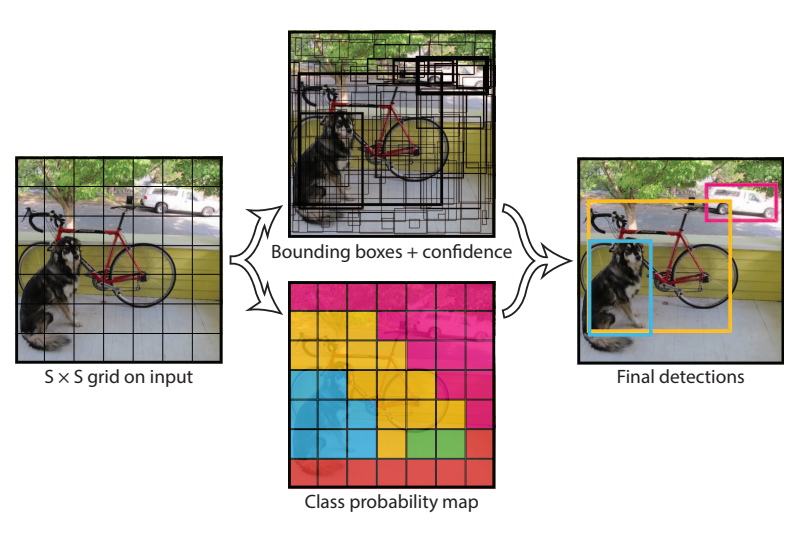
\includegraphics[height=6cm]{images/yolo.png} %
	\caption{\textit{YOLO} modelis \cite{redmon2016you}}%
	\label{fig:example}%
\end{figure}

Katrs ierobežojošais logs satur piecas prognozes: koordinātes, kas norāda loga centru attiecībā pret režģa šūnām, loga augstuma un platuma vērtības un pārliecības vērtību. Katra šūna prognozē nosacītās klašu varbūtības. Neatkarīgi no atrasto ierobežojošo logu skaita, katrai šūnai tiks piešķirta tikai viena klase.

Pētījumā \cite{redmon2016you} minētajai standarta \textit{YOLO} sistēmai ir 24 konvolūcijas slāņi, kam seko 2 pilnīgi savienotie slāņi. Pirmie konvolūcijas slāņi iegūst attēlu īpašības, kamēr pilnīgi savienotie slāņi prognozē objektu varbūtības un koordinātes.

\begin{figure}[h]%
	\centering
	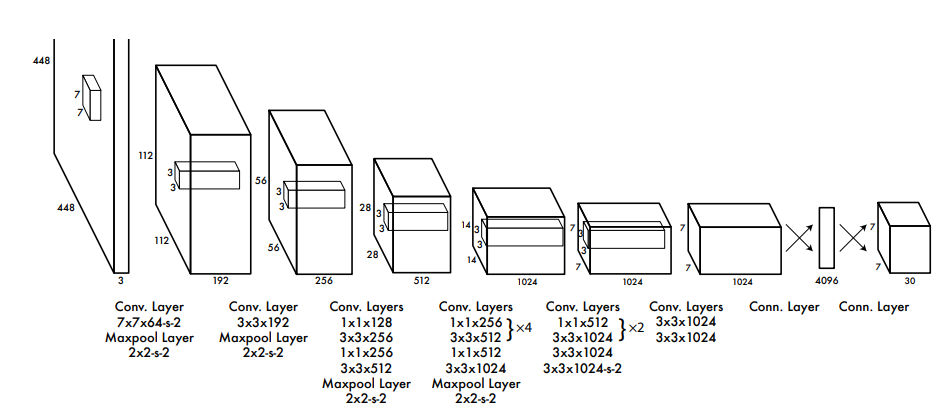
\includegraphics[height=7cm]{images/yoloarch.png} %
	\caption{\textit{YOLO} tīkla arhitektūra \cite{redmon2016you}}%
	\label{fig:example}%
\end{figure}
\newpage
Lai gan \textit{YOLO} ir labs un ātrs risinājums objektu detektēšanā, tam ir savi ierobežojumi:
\begin{itemize}
	\item Šī sistēma uzliek telpiskus limitus ierobežojošo logu prognozēm, jo katra režģa šūna prognozē tikai divus logus un katrai šūnai var piešķirt tikai vienu klasi. Šāds telpisks ierobežojums, limitē cik tuvumā esošus objektus \textit{YOLO} modelis var atrast. Tas nozīmē, ka sistēmai problēmas sagādā mazi objekti, kas atrodas grupās, piemēram, putni.
	\item Līdzīgi kā citas objektu detektēšanas metodes, \textit{YOLO} iemācās veikt ierobežojošo logu prognozes balstoties uz apmācības datiem, kas nozīmē, ja objektu detektēšana jāveic attēliem ar neierastiem izmēriem vai uzstādījumiem, \textit{YOLO} var būt grūti izšķirt objektus šajos attēlos.
	\item Attēlā 2.2 ir redzams, ka tīkla arhitektūrā ir vairāki apvienošanas slāņi (\textit{Maxpool layer}), kas nozīmē, ka ierobežojošo logu prognozēšanā tiek izmantotas salīdzinoši zemas kvalitātes (no angļu val. \textit{coarse}) īpašības. 
	\item Apmācības laikā izmantotā \textit{loss} funkcija pieņem, ka kļūdas mazajos ierobežojošajos logos ir tik pat būtiskas kā kļūdas lielajos logos, kas nav labs risinājums. Mazai kļūdai lielā logā ir maza ietekme, taču tikpat mazai kļūdai mazā logā var būt liela ietekme uz pārliecības rezultātiem. 
\end{itemize}   

\subsubsection{Faster-RCNN (\textit{Faster Region-Based Convolutional Neural Network})}
\textit{Faster-RCNN} ir objektu detektēšanas sistēma, kas sastāv no diviem tīkliem: reģionu noteikšanas tīkla (no angļu val. \textit{region proposal network}) jeb RPN, kas veido reģionu priekšlikumus, un no tīkla, kas šiem reģioniem veic objektu detektēšanu. RPN atgriež vairākus logus jeb priekšlikumus, kurus novērtēs klasifikators un regresors, lai noteiktu objektu esamību konkrētajā logā.

\begin{figure}[h]%
	\centering
	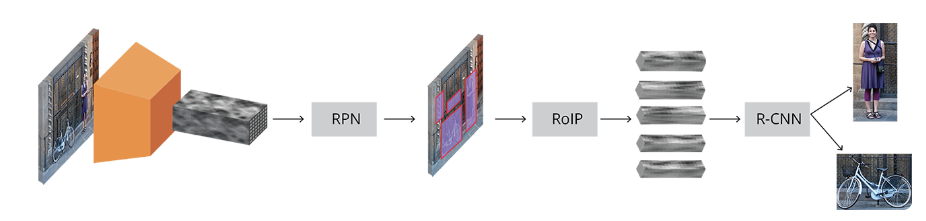
\includegraphics[height=3.5cm]{images/fastercnnarch.png} %
	\caption{\textit{Faster R-CNN} arhitektūra \cite{fasterrcnn}}%
	\label{fig:example}%
\end{figure}
\textit{Faster R-CNN} sistēmai ir salīdzinoši sarežģīta arhitektūra. Neiedziļinoties sīkumos, šī modeļa arhitektūra (attēls 2.3) sākas ar attēlu no kura ir nepieciešams iegūt: sarakstu ar ierobežojošajiem logiem, katram loga marķējumu (klases nosaukums) un katra marķējuma un ierobežojošā loga varbūtību. 

Ievades attēls ir vairākdimensiju masīvs, kuru padod ievadē konvolūcijas neironu tīklam līdz tiek iegūta īpašību karte. Pēc īpašību kartes iegūšanas, tā tiek nodota RPN. Izmantojot šīs īpašības, tīkls meklē iepriekš definētu skaitu ar reģioniem (ierobežojošajiem logiem, kurus sauc par \textit{anchors}), kuri var saturēt objektus (RPN nav svarīgi noskaidrot kādas klases objekts atrasts, tikai vai reģionā ir kāds objekts vai reģions satur tikai fona informāciju).  Šie reģionu logi ir fiksēta izmēra ierobežojošie logi, kuri ir vienmērīgi izvietoti attēla robežās. Pēc tam kad iegūts saraksts ar iespējamiem objektiem un to atrašanās vietām attēlā, detektēšanas problēma paliek krietni vienkāršāka. Izmantojot no konvolūcijas neironu tīkla iegūtās īpašību kartes un reģionu logus ar atbilstošajiem objektiem, pielieto RoI (no angļu val. Region of Interest) apvienošanu.
\begin{figure}[h]%
	\centering
	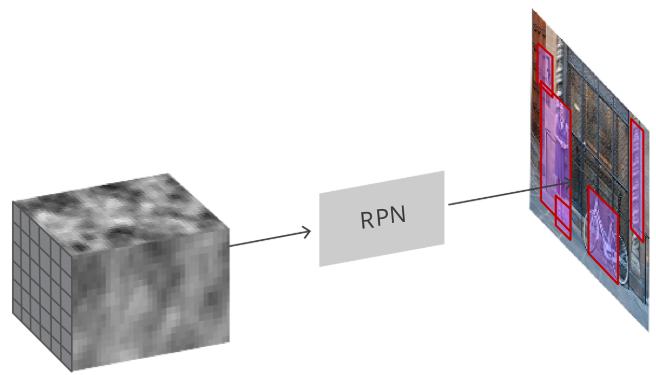
\includegraphics[height=5cm]{images/rpnstep.png} %
	\caption{RPN arhitektūra. RPN ievadē saņem no CNN atgriezto īpašību karti un attēlā ģenerē reģionu priekšlikumus. \cite{rpnarch}}%
	\label{fig:example}%
\end{figure}
Pēc RPN soļa ir iegūti vairāki prognozētie objekti, taču nav zināms kāda ir šo objektu klase. Vienkāršākais veids kā katram reģionam atrast klasi ir, samazināt šo reģionu un padot apmācītam tīklam, kas izmantojot iepriekš iegūtās attēla īpašības varēs risināt klasifikācijas problēmu, taču šāds risinājums nav efektīvs. Lai veiktu šāda veida klasifikāciju 1000 priekšlikumiem, tiks patērēts daudz laika un skaitļošanas resursu. Šo problēmu, \textit{Faster R-CNN} izstrādātāji risina vai vismaz samazina, izmantojot RoI apvienošanu \cite{roipooling}, ņemot iepriekš iegūto īpašību karti un iegūtos reģionus. 

Pēc RoI apvienošanas soļa seko R-CNN daļa, kas klasificē reģionu logu saturu vai arī atmet to, norādot reģiona marķējumā, ka tas ir fons. Kā arī R-CNN tīkls atjauno reģionu ierobežojošo logu koordinātes, lai ierobežojošais logs precīzāk pārklātu objektu. R-CNN izmanto katra piedāvātā reģiona īpašību karti, saplacina (no angļu val. \textit{flattens}) to un izmanto divus pilnīgās savienošanas slāņus ar ReLU kā aktivizācijas funkciju un atgriež objekta varbūtību un atjaunotā ierobežojošā loga robežas.

\begin{figure}[h]%
	\centering
	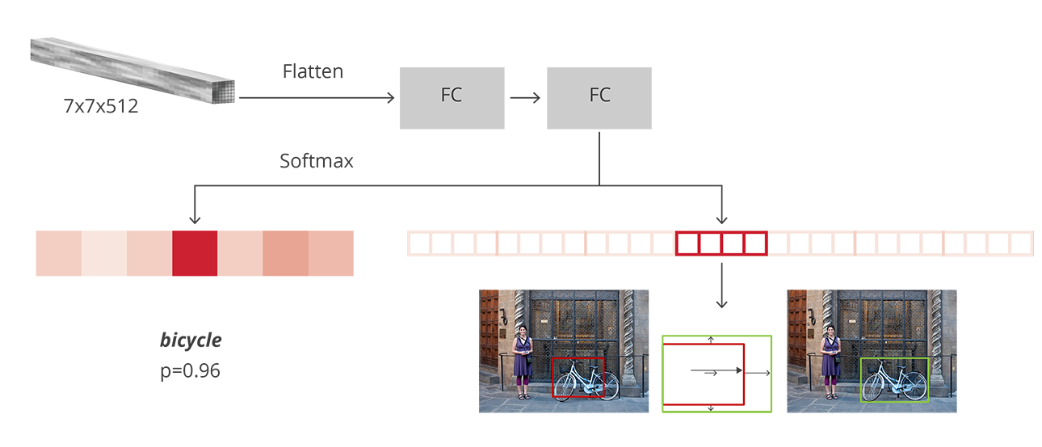
\includegraphics[height=5cm]{images/rcnnarch.png} %
	\caption{R-CNN arhitektūra \cite{fasterrcnn}}%
	\label{fig:example}%
\end{figure}

Līdzīgi kā pēc RPN soļa, pēc R-CNN soļa ir iegūti objekti, kuriem ir atrastas klases un kurus ir nepieciešams papildus apstrādāt. Lai  katram reģionam pielietotu ierobežojošo logu labojumus, tiek ņemts vērā kuras klases atrastā varbūtība bija ar visaugstāko vērtību (ja reģiona augstākā varbūtība ir klase "fons", tad šis reģions tiek ignorēts). Pēc gala objektu iegūšanas un "fona" objektu atmešanas, tiek pielietots uz klasēm balstīts NMS (\textit{non-maximum suppression}), lai novērstu vienas un tās pašas objekta instances detektēšanu vairākos reģionos \cite{hosang2017learning}.

\subsubsection{SSD (\textit{Single Shot MultiBox Detector})}

Īsumā, \textit{SSD} galvenā ideja ir tāda, ka tiek izmantots tikai viens neironu tīkls, kas padara risinājumu ātru un nav nepieciešamība pēc reģionu priekšlikumiem. Tā vietā, tiek izmantotas dažādi ierobežojošie logi, kuri tiek mainīti prognožu izdarīšanas laikā. Pētījums par \textit{SSD} kļuva pieejams 2016. gadā \cite{liu2016ssd} un šī detektēšanas sistēma uzstādīja jaunus rekordus veiktspējā un precizitātē objektu detektēšanas uzdevumu veikšanai. Lai labāk saprastu \textit{SSD} ir vērtīgi izskaidrot šīs sistēmas pilno nosaukumu:
\begin{itemize}
	\item \textit{\textbf{Single Shot}} : tas nozīmē, ka objektu lokalizācijas un klasifikācijas uzdevumus tiek veikts neironu tīkla slāņiem izejot cauri vienu reizi;
	\item \textit{\textbf{MultiBox}} : ir ierobežojošo logu regresijas tehnika, kuru izveidoja pētnieki, kas strādāja ar pie \textit{SSD} izveides;
	\item  \textit{\textbf{Detector}} : \textit{SSD} sistēmā neironu tīkls ir objektu detektors, kas arī klasificē detektētos objektus;
\end{itemize}
\newpage
\begin{figure}[h]%
	\centering
	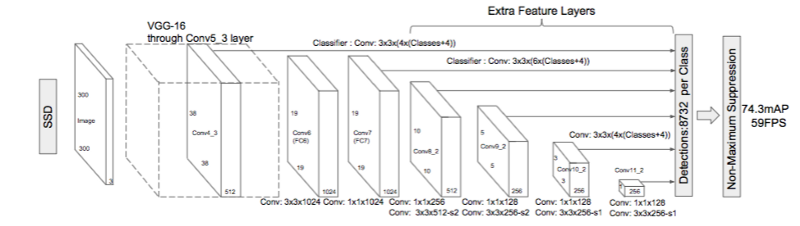
\includegraphics[height=4.5cm]{images/ssdarch.png} %
	\caption{SSD arhitektūra \cite{ssdarch}}%
	\label{fig:example}%
\end{figure}

Attēlā 2.6 ir attēlota \textit{SSD} arhitektūra, kur parādīts, ka šī objektu detektēšanas sistēma ir balstīta uz \textit{VGG Net} arhitektūru, taču netiek izmantoti standarta arhitektūras pilnīgi savienotie slāņi. \textit{VGG Net} neironu tīkla arhitektūra tiek izmantota kā \textit{SSD} bāze, jo tā darbojas ar augstu veiktspēju attēlu klasifikācijas uzdevumu veikšanā \cite{simonyan2014very}. Tai vietā, lai \textit{SSD} izmantotu pilnīgi savienotos slāņus no standarta \textit{VGG Net} konfigurācijas, tiek izmantoti papildus konvolūcijas slāņi, lai būtu iespējams iegūt attēla īpašības dažādos attēla izmēros un samazinātu katra nākamā slāņa ievadē saņemto attēlu izmēru. 

\textit{MultiBox} ir ierobežojošo logu regresijas metode, kas balstīta uz \textit{SSD} izstrādātāju pētījumu par objektu ierobežojošo logu koordināšu priekšlikumiem \cite{szegedy2014scalable}, kur nav zināmas objektu klases. \textit{MultiBox} \textit{loss} funkcija apvieno divas objektu detektēšanas mērvienības: \textit{confidence loss} un \textit{location loss}. \textit{Confidence loss} mēra, cik pārliecināts ir tīkls, ka aprēķinātais ierobežojošais logs satur objektu. \textit{Location loss} mēra cik tālu no tīkla prognozētajiem ierobežojošajiem logiem atrodas \textit{ground-truth} ierobežojošie logi apmācības datos. \textit{MultiBox loss} aprēķina sekojoši:

\begin{equation}
\var{multibox_loss}
= \var{confidence_loss}
+ \var{alpha}
* \var{location_loss}
\end{equation}
\textit{Alpha} minētajā vienādojumā palīdz balansēt \textit{location loss} vērtību. Līdzīgi kā citām dziļās mašīnmācīšanās sistēmām, ir nepieciešams atrast vienādojuma parametrus, kas vislabāk samazina \textit{loss} funkciju, tādējādi pietuvinot tīkla prognozes \textit{ground-truth} vērtībām.

\textit{MultiBox} pētnieki veidojot šo metodi ieviesa jaunu terminu \textit{priors}. \textit{Priors} ir iepriekš aprēķināti, fiksēta izmēra ierobežojošie logi (\textit{Faster R-CNN} sistēmā šos logus sauc par \textit{anchors}), kas cieši sakrīt ar \textit{ground-truth} ierobežojošo logu izvietojumu. Balstoties uz šiem iepriekš aprēķinātajiem ierobežojošiem logiem, \textit{MultiBox} tos izmanto kā prognozes un mēģina regresēt tuvāk \textit{ground-truth} ierobežojošajiem logiem. Beigās \textit{MultiBox} saglabā tikai labākās prognozes ar minimizētām \textit{location loss} un \textit{confidence loss}. 

\textit{SSD} pētījumā ir veikti uzlabojumi standarta \textit{MultiBox} sistēmai, kas padara šo objektu detektēšanas sistēmu vēl spējīgāku lokalizēt un klasificēt objektus. \textit{SSD} katra īpašību kartes šūna ir savienota ar dažādu izmēru un dažādu proporciju ierobežojošajiem logiem (\textit{priors}). Šie logi ir manuāli izvēlēti, kas, teorētiski, ļauj \textit{SSD} darboties ar dažādi konfigurētiem ievades datiem. Pieņemot, ka ir definēts \textit{c} skaits klašu, katrai īpašību kartes šūnai ir definēts \textit{b} skaits ierobežojošo logu un īpašību kartes izmērs ir \textit{f}, \textit{SSD} aprēķinātu \textit{f * b * (4 + c)}
vērtības šai īpašību kartei. 

\begin{figure}[!htb]
	\minipage{0.32\textwidth}
	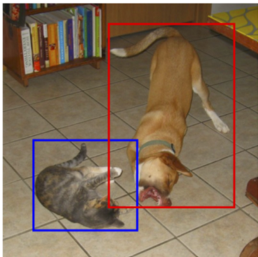
\includegraphics[width=\linewidth]{images/ssdgtboxes.png}
	\caption{Attēls ar \textit{ground-truth} logiem \cite{liu2016ssd}}
	\endminipage\hfill
	\minipage{0.32\textwidth}
	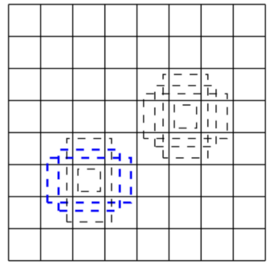
\includegraphics[width=\linewidth]{images/ssd88featmap.png}
	\caption{8 x 8 izmēra īpašību karte \cite{liu2016ssd}}
	\endminipage\hfill
	\minipage{0.32\textwidth}%
	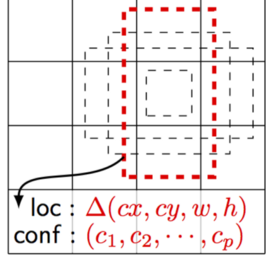
\includegraphics[width=\linewidth]{images/ssd44featmap.png}
	\caption{4 x 4 izmēra īpašību karte \cite{liu2016ssd}}
	\endminipage
\end{figure}

Attēlā 2.7 ir parādīts, ka apmācības laikā \textit{SSD} ir tikai nepieciešams ievades attēls un \textit{ground-truth} logi, kas atspoguļo objektus attēlā. Izmantojot konvolūcijas principus, tiek novērtēti daži ierobežojošie logi, dažādos attēla mērogos un tie tiek uzglabāti īpašību kartēs ar dažādiem izmēriem (attēlā 2.8 ir parādīta 8x8 izmēra īpašību karte un attēlā 2.9 4x4 izmēra īpašību karte). Katram logam aprēķina formas nobīdi no patiesās un pārliecības vērtības katrai objektu kategorijai (attēlā 2.9 c1,c2,...,cp). Apmācības laikā, definētie logi tiek pieskaņoti \textit{ground-truth} logiem. Piemēram, attēlā 2.7 parādīts, ka divi ierobežojošie logi ir pieskaņoti kaķim un sunim. Modeļa \textit{loss} (modeļa kopējā precizitāte ņemot vērā apmācības un validācijas datus) ir svērtā summa starp \textit{localization loss} un \textit{confidence loss}. 

Līdzīgi \textit{Faster-RCNN}, arī \textit{SSD} kā vienu no pēdējiem soļiem tīkla izpildes laikā izmanto \textit{non-maximum suppression} (NMS). Pēc detektēšanas soļa iegūtie logi tiek šķiroti pēc norādīta sliekšņa, kas atkarīgs no \textit{confidence loss} vērtības. Tikai labākos logus saglabā un pārējie (mazāks \textit{confidence loss} par sliekšņa vērtību) tiek atmesti. NMS pielietošana nodrošina, ka tikai labākās logu prognozes tīkls saglabās un trokšņainās atmetīs.
 \newpage
\begin{figure}[h]%
	\centering
	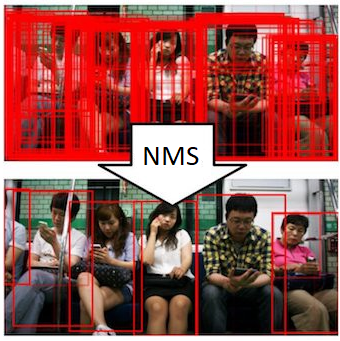
\includegraphics[height=4cm]{images/nms.png} %
	\caption{\textit{Non-maximum supression} piemērs \cite{liu2016ssd}}%
	\label{fig:example}%
\end{figure}

\textit{SSD} pētījumā \cite{liu2016ssd} ir aprakstīti novērojumi par sistēmas darbību:
\begin{itemize}
	\item Jo vairāk iepriekš definētie logi, jo precīzāk notiek detektēšana, taču tas negatīvi ietekmē sistēmas ātrumu;
	\item Izmantojot \textit{MultiBox} vairākos slāņos, sistēma objektu detektēšanu veic precīzāk, jo detektors tad darbojas ar dažādu izšķirtspēju īpašībām;
	\item \textit{SSD} mēdz jaukt objektus, kam ir līdzīgas klases (piemēram, dzīvnieki ar 4 kājām);
	\item \textit{SSD} vāji strādā ar maziem objektiem, jo tie var neuzrādīties visās īpašību kartēs. Palielinot ievades attēlu izšķirtspēju ir iespējams samazināt šo problēmu.
\end{itemize}

Ņemot vērā tikai pētījumos \cite{redmon2016you,ren2015faster,liu2016ssd} pieejamo informāciju, dotajā brīdī, \textit{Faster R-CNN} ir labākā objektu detektēšanas sistēma, ja vērā ņem tikai precizitātes vērtējumus un lietotājam ir pieejami neierobežoti skaitļošanas resursi. Ja lietotājiem ir ierobežoti skaitļošanas resursi, \textit{SSD} ir labākais ātruma un precizitātes kompromiss. Ja par precizitāti nav jāuztraucas, bet ir vēlme pēc ļoti ātras sistēmas, tad labākais variants ir \textit{YOLO}. Lai gan \textit{Faster R-CNN} labāk par pārējiem spēj atrast maza izmēra objektus, sistēma ir lēna un nenodrošina reālā laika detektēšanu. Gan \textit{YOLO}, gan \textit{SSD} sistēmas nodrošina reālā laika objektu detektēšanu, kas ir nepieciešams šī darba ietvaros. Ņemot vērā augstāk minēto informāciju, pētījuma ietvaros radītais risinājums izmantos \textit{SSD} objektu detektēšanas sistēmu, jo tā ir labākā precizitātes un ātruma apvienojums un apmācību ir iespējams veikt ar lietotājiem pieejamākām ierīcēm. 

\section{Sekošanas algoritmi}
Pēc objektu detektēšanas metodes izvēlēšanās, šī pētījuma ietvaros ir nepieciešams apskatīt sekošanas risinājumus, kuru izmantot gala risinājumā. Lai veiksmīgi veiktu cilvēku plūsmas analīzi, ar izvēlēto objektu detektēšanas metodi vien nepietiek, objektiem ir arī jāseko. Šādā risinājumā ir vērtīgi ieviest sekošanas risinājumu sekojošu iemeslu dēļ:
\begin{itemize}
	\item Sekošanas algoritmi darbojas ātrāk kā detektēšanas algoritmi. Šādu argumentu var izskaidrot ar to, ka sekojot objektam, kas jau ir atrasts iepriekšējā kadrā, sistēmai ir pieejama informācija par objekta attēlojumu, atrašanās vietu, kustības virzienu un kustības ātrumu. Sekošanas algoritms izmantos visu šo informāciju, lai nepazaudētu objekta atrašanās vietu, kamēr objektu detektēšanas algoritmam katrs katrs ir jāapstrādā no jauna.
	\item Sekošanas algoritmi ir kā drošības tīkls gadījumā, ja detektēšanas risinājumi vairs nevar atrast kādu no iepriekšējos kadros noteiktajiem objektiem. Piemēram, ja starp objektu un video kameru nostājas šķērslis, tas detektēšanas risinājumiem sagādās pamatīgas problēmas, kamēr labs sekošanas risinājums nepazaudētu objekta atrašanās vietu.
	\item Sekošanas algoritmi veido savienojumus starp video kadriem, tādā veidā saglabājot objekta identitāti.
\end{itemize}

Sekošanas mērķis ir atrast objektu dotajā video kadrā, pieņemot, ka objektam ir veiksmīgi sekots visos iepriekšējos kadros vai dotajā kadrā pirmo reizi atrasta šī objekta instance. Tā kā objektam ir sekots līdz dotajam kadram, ir zināms, ka objekts kustas, kas nozīmē, ka ir zināmi kustības modeļa parametri. Kustības modeli veido iepriekšējos kadros noteiktā objekta atrašanās vieta un ātrums. Nezinot neko citu kā kustības modeļa parametrus jau ir iespējams izteikt diezgan precīzu minējumu kur dotajā kadrā varētu atrasties objekts. Risinot sekošanas problēmu video fragmentos, ir pieejama informācija par vairāk kā tikai objekta kustību ir zināms arī objekta izskats visos iepriekšējos kadros. Zinot objekta izskatu, ir iespējams veidot izskata modeli, šādu modeli var izmantot, lai precizētu objekta atrašanās vietu pēc tam, kad balstoties uz kustības modeli ir izdarīts minējums par aptuveno objekta atrašanās vietu. Ja objekts ir vienkāršs un starp kadriem izskatu nav mainījis, tad izskata modeli var izmantot kā veidni, kuru meklēt jaunajā kadrā. Diemžēl, objekta izskats var pamatīgi mainīties, lai cīnītos ar šo problēmu modernie sekošanas risinājumi izmanto izskata modeli kā klasifikatoru, kurš tiek apmācīts algoritma izpildes laikā. 

Gala risinājuma izstrādes laikā tika apskatīti \textit{OpenCV} programmatūrā piedāvātie sekošanas algoritmi: \textit{Multiple Instance Learning} (MIL) un \textit{AdaBoost} kā arī \textit{SiamFC} sekošanas algoritms, kas neietilpst \textit{OpenCV} bibliotēkā, bet ir aprakstīts Luka Bertinetto pētījumā \cite{bertinetto2016fully}.

\subsubsection{Multiple Instance Learning sekošanas algoritms}
\textit{Multiple Instance Learning} jeb MIL sekošanas algoritma apmācības laikā, apmācības datu piemēri algoritmam ir nodoti kopās, kuras dēvē par "somām" un marķējumi (no angļu val. \textit{labels}) tiek piešķirti visai somai un nevis individuālām instancēm. Ja soma ir marķēta kā pozitīva, tad tiek pieņemts, ka somā ir vismaz viens pozitīvs piemērs, pretējā gadījumā soma ir marķēta kā negatīva. Objektu detektēšanas problēmu risināšanā, pozitīva soma var saturēt vairākus iespējamos ierobežojošos logus ap kādu iepriekš atrastu objektu. Pēc tam šīs somas nodod apmācības algoritmam un šī algoritma uzdevums ir atrast kura instance katrā pozitīvajā somā ir visprecīzākā. 

MIL sekošanas algoritma sistēma sastāv no trīs komponentēm: attēla reprezentācijas, izskata modeļa un kustības modeļa. Izskata modelis sastāv no diskriminējoša (no angļu val. \textit{discriminative}) klasifikatora kas ir spējīgs atgriezt varbūtību $ p(y = 1|x) $, kur \textit{x} ir attēla apgabals un \textit{y} ir binārs mainīgais, kas norāda vai  interesējošais objekts atrodas attēla apgabalā. Katrā solī \textit{t}, sekošanas algoritms saglabā objekta atrašanās vietu $ l_t $. Katrā nākamajā kadrā tiek izgriezti vairāki attēla apgabali $ X^s = [x|s > ||  l(x) - l_{t-1}]$, kas atrodas dotajā brīdī atrastā objekta meklēšanas rādiusā \textit{s} un aprēķina $p(y|x)$ visiem \textit{x}. Pēc tam tiek atjaunota sekošanas algoritma atrašanās vieta:

\begin{equation}
l_t = l (argmax_{x} p(y|x))
\end{equation}

Tas nozīmē, ka katrā kadrā netiek saglabātas mērķu atrašanās vietas, tā vietā tiek izmantots kustības modelis un  sekošanas algoritma atrašanās vieta tiek salīdzināta ar iepriekšējā iterācijā atrasto atrašanās vietu.
\begin{equation}
p(l_t|l_t-1) \infty 
\begin{cases} 
1 & if ||l_t - l_{t-1}|| < s \\
0 & otherwise
\end{cases}
\end{equation}
Lai ietaupītu skaitļošanas resursus un vienkāršības nolūkos šis algoritms neizmanto citu kustības informāciju kā objekta izmēru maiņas vai rotācijas informāciju.

Pēc sekošanas algoritma atrašanās vietas atjaunošanas ir nepieciešams atjaunot izskata modeli. Tiek iegūti attēla apgabali $ X^r =
x|r > ||l(x)-l_t||
$ un ja \textit{r} (apgabala rādiuss) atrodas sekošanas algoritma rādiusā, tad doto attēlu apgabalu somu marķē kā pozitīvu. Lai iegūtu negatīvos piemērus, tiek izgriezti attēla apgabali apļveida reģionā\\ $X^{r,\beta} = 
x|\beta > || l(x) - l_t|| > r$. Šādi iegūti attēlu apgabali dos ļoti lielu negatīvo piemēru datu kopu, tāpēc no šīs kopas kā negatīvos piemērus izmantos tikai gadījuma lieluma apakškopu ar attēlu apgabaliem\cite{babenko2009visual}.\\ MIL sekošanas algoritmu var aprakstīt ar pseidokodu:
\begin{algorithm}
	\caption{MIL sekošana}\label{euclid}
	\begin{algorithmic}[1]
		\item[\textbf{Ievades dati:}] Attēls
		\State Izgūst attēla apgabalus, $ 
		X^s = \left\{\begin{array}{lr}
		x|s > || l(x) - l_{t-1} ||
		\end{array}\right\} $
		\State Izmanto MIL klasifikatoru, lai noteiktu $p(y=1|x)$ katram \textit{x}
		\State Atjauno sekošanas algoritma atrašanās vietu $l_t = l (argmax_{x} p(y|x))$
		\State Izgriež pozitīvo un negatīvo piemēru attēlu apgabalus
		\State Atjauno MIL izskata modeli
	\end{algorithmic}
\end{algorithm}
\subsubsection{AdaBoost sekošanas algoritms}
Pieņemot, ka detektējamais objekts jau ir atrasts, \textit{AdaBoost} sekošanas algoritms pieņem, ka dotais attēla reģions ir pozitīvs piemērs sekošanas algoritmam. Lai iegūtu negatīvos piemērus, tiek izgūti tāda paša izmēra reģioni no atrastā objekta apkārtnes. Šos piemērus izmanto, lai izveidotu vairākas \textit{boosting} algoritma iterācijas, kas iegūtu stabilu sekošanas modeli. Šie soļi gan ir nepieciešami tikai lai inicializētu sekošanas algoritmu, pats sekošanas solis ir balstīts uz veidņu (no angļu val. \textit{template}) sekošanas principu \cite{hager1998efficient}. Katrā reģionā klasifikators veic novērtējumu un iegūst pārliecības vērtības. Pārliecību karti analizē un pārvieto sekošanas algoritmu uz reģionu ar augstāko pārliecības novērtējumu. Pēc tam, kad objekts atrasts jaunajā kadrā, klasifikatoru ir nepieciešams atjaunot, lai tas varētu izšķirt objekta izskata izmaiņas vai lai tas varētu atšķirt fonu no meklējamā objekta. Reģions kurā atrodas sekošanas algoritms tiek padots klasifikatoram kā pozitīvais piemērs un apkārtējie reģioni tiek padoti klasifikatoram kā negatīvie piemēri priekš klasifikatora atjaunošanas. Apstrādājot jaunus kadrus, visa minētā procedūra tiek atkārtota un klasifikators ir spējīgs pielāgoties iespējamajām objekta izskata izmaiņām un fona trokšņiem.

\textit{AdaBoost} jeb \textit{Adaptive Boosting} algoritms spēj ģenerēt klasifikatorus, kurus var efektīvi atjaunināt, iteratīvi padodot tam jaunus piemērus. Lai labāk saprastu šo algoritmu ir nepieciešams izskaidrot sekojošas definīcijas:
\begin{itemize}
	\item \textbf{Vājš klasifikators:} Klasifikators, kas darbojas tikai nedaudz labāk kā nejauša minēšana (piemēram, bināru lēmumu pieņemšanā, kļūdai jābūt mazākai par 50\%). Vāja klasifikatora izdarīto prognozi apzīmē ar $h^{weak}$.
	\item \textbf{Selektors:} Pieņemot, ka ir kopa ar vājiem klasifikatoriem, kuri apzīmēti ar $H^{weak} = [h^{weak}_1,...,h^{weak}_M]$, selektors izvēlas vienu no šiem klasifikatoriem $h^{sel}(x) = h^{weak}_m(x)$, kur \textit{m} ir izvēlēts atkarībā no optimizācijas kritērija. Piemēram, var izmantot katra vājā klasifikatora kļūdu $e_i$ un izvēlēties mazāko, tas nozīmē, ka $m = argmin_ie_i$.
	\item \textbf{Spēcīgs klasifikators:} Pieņemot, ka ir kopa ar vājiem klasifikatoriem, spēcīgs klasifikators tiek aprēķināts kā selektoru lineāra kombinācija. 
\end{itemize}

\textit{Boosting} algoritma galvenā doma ir selektoru ieviešana. Tie tiek nejauši inicializēti un katrs satur atšķirīgu īpašību no vājajiem klasifikatoriem. Kad algoritmam tiek padots jauns piemērs apmācībai, katra selektora vājie klasifikatori tiek atjaunoti. Pēc katra algoritma iterācijas ir pieejams spēcīgs klasifikators, bet vissliktāko vājo klasifikatoru aizstāj ar jaunu, nejauši izvēlētu.

\subsubsection{SiamFC sekošanas algoritms}
\textit{SiamFC} sekošanas algoritms piedāvā apmācīt funkciju $f(z,x)$, kas salīdzina vienāda izmēra parauga attēlu \textit{z} ar piedāvāto attēlu \textit{x} un atgriež novērtējumu cik ļoti abi attēli attēlo to pašu objektu. Šādu apmācību sauc par līdzības apmācību (no angļu val. \textit{similarity learning}). Lai atrastu objekta pozīciju jaunajā attēlā, tiek izsmeļoši pārbaudītas visas iespējamās atrašanās vietas un izvēlēts kandidāts ar augstāko līdzību iepriekšējā kadrā redzētajam objektam. Minēto funkciju \textit{f} apmāca, izmantojot datu kopas ar video, kuros norādīta objektu kustību trajektorija. 

Tā kā datorredzes problēmu risināšanai veiksmīgi tiek izmantoti konvolūciju neironu tīkli, tos iespējams pielietot arī šajā gadījumā. Konvolūcijas neironu tīkls tiks izmantots kā funkcija \textit{f}. Līdzības apmācību, izmantojot konvolūcijas neironu tīklus, parasti veido izmantojot Siāmas (no angļu val. \textit{Siamese}) arhitektūras \cite{taigman2014closing,bromley1994signature}. Siāmas tīkli abiem ievades attēliem veic identisku transformāciju $\phi$ un apvieno iegūtās reprezentācijas citā funkcijā \textit{g}, izmantojot sakarību $f(z,x) = g(\phi(z),\phi(x))$.

\begin{figure}[h]%
	\centering
	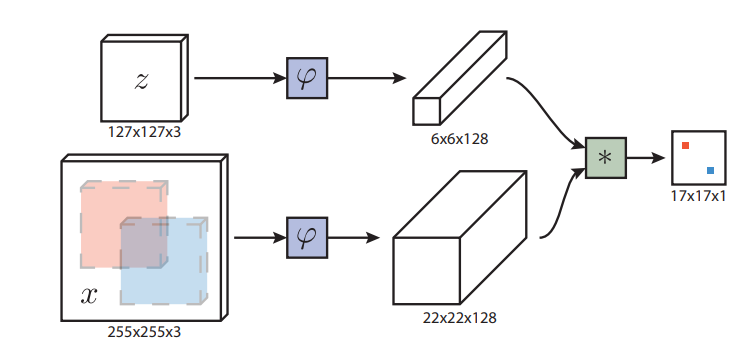
\includegraphics[height=4cm]{images/siamfcarch.png} %
	\caption{Pilnīgās konvolūcijas Siāmas arhitektūra \cite{bertinetto2016fully}}%
	\label{fig:example}%
\end{figure} 

Attēlā 2.26 ir redzama pilnīgās konvolūcijas Siāmas arhitektūra, ko izmanto šis sekošanas algoritms. Izvades dati ir rezultātu karte ar skalārām vērtībām, kuras dimensiju skaits ir atkarīgs no ievades attēla \textit{x} izmēra. Attēlā parādītajā rezultātu kartē ar sarkano un zilo pikseli ir atzīmētas vietas, kuras satur līdzības ievades attēlos.  

Sekošanas laikā, algoritms izmanto attēlu, kurā atzīmēta sekošanas mērķa atrašanās vieta iepriekšējā kadrā. Izmantojot augstākās rezultātu kartes vērtības un neironu tīkla parametrus, ir iespējams aprēķināt aptuveno objekta pārvietojumu starp kadriem. Kad ir noteikta aptuvenā atrašanās vieta, tiek pielietots konvolūcijas neironu tīkls, kas meklēs objektu dažādos izmēros objekta apvidū dotajā kadrā.
